\documentclass[11pt,captions=tableheading]{scrartcl}
\setcounter{errorcontextlines}{50}
\setlength\parindent{0pt}
\usepackage{etex}
%Sprache, Trennung
\usepackage[utf8]{inputenc} %Textsatzvodoo
\usepackage[T1]{fontenc} % Textsatzvodoo, beide notwending, da sonst ö ä ü aus pdf kopieren nicht geht
\usepackage[ngerman]{babel}

%Font, Farben
\usepackage{lmodern}	% Schrift, die besser gesetzt wird
\usepackage{xcolor} %Ermöglicht Ändern der Schriftfarbe, neuer als color-package
%\usepackage{marvosym,dsfont}

%Mathe Richtlinien
\usepackage{amsmath}

%Captions, all kiiind of shit
\usepackage[rightcaption]{sidecap}
\usepackage{caption}

%Abbildungen
\usepackage{wrapfig,subfigure,graphicx,rotating}
\usepackage[percent]{overpic} %Schrift in Bild einfügen
\usepackage{float} % einbinden von Grafiken

%Tabellen
\usepackage{array, adjustbox, tabularx,threeparttable,booktabs}
\usepackage{longtable} % Große Tabellen
\usepackage{multirow, multicol} % Zellen in Tabellen vertikal und horizontal verbinden

%Gemischt
\usepackage[pdfborderstyle={/S/U/W 0.5}]{hyperref}
\usepackage{capt-of,todonotes, import, setspace,comment, url, eurosym, pdflscape,natbib,scrpage2, }


%\usepackage[style=authoryear]{biblatex}

\hypersetup{pageanchor=false}
\hyphenation{quell-offenen klein-skaligen}
\hyphenation{Videobeo-bachtungs-plattform}
\newcommand{\re}[1]{\ensuremath{#1\cdot	10^{5}}}

\selectlanguage{ngerman}

\usepackage{geometry}
\geometry{verbose,a4paper,lmargin=25mm,rmargin=25mm,bmargin=25mm,tmargin=25mm}

\captionsetup{position=top, singlelinecheck=false, justification =, margin=8pt,labelfont={small,bf}, aboveskip=0pt,indent=0pt}
\setcapindent{0pt}
\addtokomafont{caption}{\small}

\onehalfspacing

\setlength\abovecaptionskip{10pt}

%Benutzerbefehle
\newcolumntype{C}[1]{>{\centering\let\newline\\\arraybackslash\hspace{0pt}}m{#1}}
\newcolumntype{L}[1]{>{\raggedright\let\newline\\\arraybackslash\hspace{0pt}}m{#1}}
\newcolumntype{R}[1]{>{\raggedleft\let\newline\\\arraybackslash\hspace{0pt}}m{#1}}

\newcommand{\kmh}{$\mathrm{kmh^{-1}}$}

\date{\today}
\title{Lokomotion}
\author{Vincent E. Focke}

\begin{document}
% % % %
\begin{titlepage}
\begin{minipage}[c]{9cm}
\vspace{0pt}
\textsc{\large Bionik: Mobile Systeme (M.Sc.)}\\
\textsc{Fakultät 5: Natur und Technik}\\
\textsc{\small Modul 1.2}\\
[0.5cm]
\underline{\large \textbf{WS 2016/17}\hspace{10.5cm} \textbf{\today}}\\
\end{minipage}
\begin{minipage}[c]{6cm}
\vspace{0pt}
%\includegraphics[width=1.1\textwidth]{Bilder/HSB_Logo}
\vspace{1cm}
\end{minipage}

\begin{center}
\vspace{5cm}


\text{\large \textbf{Lokomotion Motherfucker}}\\
[1.5cm]

\huge \bfseries Versuche terrestrische Lokomotion\\
[0.4cm]

\vfill

% Bottom of the page
\end{center}
\normalsize
{\text{\textsc{\textbf{Student:}} Vincent E. Focke}}\\
{\text{\textsc{\textbf{Leitung:}} Prof. Dr. A. Kesel}}\\
{\text{\textsc{\textbf{Betreuung:}} LB. Nils Owsianowski}}\\
\end{titlepage}
\pagenumbering{Roman}
\setcounter{page}{1}
\tableofcontents
\setcounter{tocdepth}{3}
%\listoffigures
%\listoftables
% % % %
% Kopf und Fußzeile % % % % %
\clearscrheadfoot
\pagestyle{scrheadings}
%\ohead{\headmark}
%\automark{section}
\cfoot[]{} 
\ofoot[\pagemark]{\pagemark}
% % % % % % % % % % %
\newpage
\pagenumbering{arabic}
\setcounter{page}{1}
%\section{TODO}

\textbf{Kirtley et al 1985}

knee angle and moment and changes over walking speed\\
peak knee reflexion strongly correlated wit walkin gsped\\

discussion;\\
strong correlation of cadence, stride length and velocity\\
velocity highest correlation with stance phase\\
cadence highest correlation with swing phase knee flexion

GOOD ARGUMENTATION!\\
Cadence, stride length and velocity\\
Eigenfrequency cant be changed, therefore energy is needed for decelaration and acceleration when walking faster or slower\\
walking becomes \textbf{more difficult}\\

shortening stance phase due to the fact that swing phase cant be shortened as easily as stance phase (gibt quelle 11 an, nachgucken! zitieren!)

no change in knee extension peaks, kurz vor der landung,bei 2/3 der standphase\\

Kniewinkel\\
Standphase: extension kaum verändert, flexionsmaximum steigt\\
Schuwngphase: kein große Änderung des lfexionswinkels??\\

\textbf{Kuo2007}
check cincluiso Seite 35\\
Pendulum ist ne gute theorie! aber irgendwas mit fliegender Kugel und "dnymic walking"

\textbf{whittle1996}\\
Seite 8 und 10\\
gute graphen!\\

\textbf{Danion2003}\\
Gangzyklen sind stark variabilität unterworfen\\

\textbf{Masaad-etal2007}\\
introduciotn:\\
flat walking muscles work less efficient\\
bouncy walking muscles work more but also more efficient!\\
compare walking model types on a meta-level!!!!!!!!!!!!!!!!!!!!!\\

\textbf{alexander1992}\\
introduction: why we cant walk faster!!!\\

\textbf{TLOK-069}
introduction good for robotics\\


\textbf{READ!!!}\\
Alton 1998\\
Jordan 2007\\


\subsection{MundM}
Beschriftung Abbildungsteile laufsteg und laufband
\subsection{Geschw. und Beschl Linear und Winkel}
- pur plotten\\
- angucken\\
- sinnvoll plotten\\


\subsection{Scilab}
- Einlesen Tabellen\\
- Massenschwerpunkte bestimmen\\
- Geschwindigkeiten und Beschleunigung (linear und winkel)\\
- Daten glätten, gleitender Mittelwert\\
- plotten\\
-----------------------------------------\\
- Kalibrierung der Waage\\
- Messdaten bereinigen (Drift und Nullmessung)\\
- Messdaten in Kräfte umrechnen\\
(y-Richtung Waage = x-Richtung der Videos)\\
(z-Richtung Waage = y-Richtung der Videos)\\
- Bestimmung des genauen Ortes der Bodenreaktionskraft\\
- Berechnung der inversen Dynamik\\
- Zeitliche Syncronisation der Datensätze (Startbild und Aufnahmefrequenz)\\
\clearpage

\section{Checkliste Inhalt}
\textbf{Bewertungskriterien}\\
Vorgehensweise:\\
welche Auswertungen wurden durchgeführt\\
wie viel Hingabe liegt in der Erstellung\\
wurde alles ausgewertet?\\
------------------------------------------------------\\
\textbf{Pendel}\\
Eigenfrequenz ermitteln und darstellen\\
halbe periode, da nur Schwungphase betrachtet wird\\
wirklich nur die Periodendauer vergleichen\\
am leichtesten, da Schwingung nur durch Shcwerkraft entsteht und keine Muskelkraft benötigt wird -> das mit subjektiver Wahrnehmung vergleichen (hier Skala 1-10)\\
ES GEHT NUR UM WINKEL!!\\
GESCHW. UND BESCHL. SIND NUR FÜR INVERSE KINEMATIK NOTWENDIG!!\\
------------------------------------------------------\\
\textbf{Laufband mit Laufstrecke vergleichen}\\
oberkörper betrachten\\
dazu Litertur suchen -> Vorwärtsbewegung ist kontrolliertes Fallen (KUO 2007)
macht Unterschied, ob ich tatsächlich mich fortbewege oder auf der Stelle laufe\\
das über die Winkel machen!\\
verändert sich die Armschwingungs/ Amplitude\\
wie doll ändert sich der Winkel zwischen Hüfte und Nacken (Winkel zwischen Boden und Verbindungslinie Nacken/Hüfte, am besten 0 Grad senkrecht nach oben festlegen, dann positive Winkel nach vorne, negative nach hinten!)\\
OPTIONAL!\\
Treibende Kraft aus Gravitationskraft und Oberkörperneigungswinkel berechnen\\
hier müsste eigentlich rauskommen, dass keine Kraft sich ergibt über einen Schrittzyklus, da das eine Pendelbewegung ist\\
Unterschiede zwischen Laufen auf einem Fleck (Laufband) und tatsächlicher Ortsänderung(Laufstrecke)\\
Arme hierfür getrackt!! hier wichtig: Amplitude in X-Richtung und Winkel zwischen Unter- und Oberarm angucken und vergleichen\\
------------------------------------------------------\\
\textbf{Laufstrecke}\\
Auswertung durch inverse Kinematik (Winter 2009)\\
Kräfte und Momente für alle Gelenke analysieren und interpretieren\\
Bedeutung der Daten hinsichtlich bionischer oder medizintechnischer Anwendungen\\
weitere Schlussfolgerungen (s. Winter) und mögliche weiterführende Berechnunge/Untersuchungen\\

auftretende Kräfte und Momente angucken und interpretieren\\
was kann man daraus ablesen\\
welches Kraft/moment tritt wann auf, warum ist das so?\\
das mit Kinematik koppeln\\
bei welcher Gangphase passiert was, was kann daraus gezogen werden?\\
siehe Winter: was kann man noch weiter berechnen, Ansatz der Hebelarme etc...\\
welche Auswirkung hat dieses Wissen für technische Anwendung, zum Beispiel die ideale Dämpfung\\
Robotik, was kann man für bipedales Gehen für Gangmuster (central pattern generators - CPG) aus den Untersuchungen ziehen -> Robotik, Medizintechnik, Exoskelette\\



------------------------------------------------------\\
Anwendung auf andere Fortbewegungssysteme/ mögl. Anwendungen\\
Robotik, 4/6/8 Beine\\
Exoskelette Programmierung für natürlich Unterstützung des Menschen\\
------------------------------------------------------\\
auf Fehlen der Statistik eingehen\\
kurz beschreiben, welche Daten notwendig wären, welche Verfahren geeignet wären\\
------------------------------------------------------\\
\textbf{Weiterführende Literatur!!}\\
\clearpage

MATERIAL UND METHODEN

Mit diesen Koordinaten werden die lineare Geschwindigkeit und Beschleunigung der Körperteile mittels Zentraldifferenz berechnet.\\
ZENTRALDIFFERENZ\\

Zur Berechnung der Winkelgeschwindigkeit und -beschleunigung sind folgende Gleichungen verwendet worden:\\
WINKELPROBLEM??\\
WIE GELÖST???\\

Alle Trajektorien, Geschwindigkeiten und Beschleunigungen wurden mittels gleitendem, gewichteten Mittelwert geglättet.\\
MITTELWERT!!!\\
DEN MÜSSEN WIR NOCH DARAUF ANWENDEN!!!\\
Für die Auswertung dir kinetischen Daten muss zunächst eine Waagenkallibration durchgeführt werden, um deren Drift zu bestimmen und die Spannungswerte mit dem Körpergewicht zu korrelieren. Das folgende Vorgehen wurde in allen drei Raumrichtungen durchgeführt: Aus einer Null-Messung ohne Belastung werden XXXX Werte gewählt und durch lineare Regression der Drift der Waage bestimmt. In einer zweiten Messung wird bei A, B, C und D kg jeweils 30~s gemessen. Nach Abzug des Drifts wird das Waagensignal für die vier Gweichte über 3000 Werte gemittelt und über diese vier Werte durch lineare Regression das Waagensignal mit Gewichten korreliert.\\
OFFSET-BERECHNUGN UND ABZUG BEI JEDER MESSUNG\\
HIER FEHLT NOCH DAS ZUSAMMENFASSEN DER KANÄLE\\


Aufbau siehe Kirltey et al\\
Inverse Kinematik\\
FELIX WAS HAST DU DA ALLES GEZAUBERT?!?!?

\textbf{Skalierung und Synchronisation!!}\\
- Bei der Skalierung wird die Datenrate der Videorate angepasst (hier also nur jeder 20.!!!! Datensatz). Gegebenenfalls muss zwischen den Datensätzen interpoliert werden.\\
- Bei der Datensynchronisation findet ein Abgleich des Videomaterials und der Bodenreaktionskräfte statt\\
\textbf{Digitalisierung des Videomaterials}\\
- Skalieren der Videoaufnahme (ACHTUNG! Referenzbild mit Maßstab erforderlich?!?!?)\\
- Tracken von allen Gelenken\\
- Segmentschwerpunkte berechnen (Fuß, Unter- und Oberschenkel)\\
\textbf{Datenfilterung (gleitender Mittelwert)}\\
- ACHTUNG! Je nach Anzahl von Stützstellen und Iterationen müssen Bilder vor und nach dem Schrittzyklus in die Digitalisierung einbezogen werden. z.B. 3 Stützstellen und eine Iteration benötigt 1 Bild vorher und ein Bild nachher, um i-1 und n+1 zu berücksichtigen.\\
\textbf{Kinetische Berechnungen (Wagenzentrum rausrechnen?)}\\
Auf der Grundlage von David A. Winter werden:\\
- Kräfte und Momente in den Gelenken berechnet\\
- Berechnung mittels inverser Dynamik\\
\section{Einleitung}

Die bipedalen Bewegungsformen des Menschen, Gehen und Laufen, sind durch ein komplexes Zusammenspiel von neuronalen, physiologischen und mechanischen Prozessen gekennzeichnet. 
Das Gangbild unterscheidet sich von Mensch zu Mensch, abhängig von Parametern wie Alter, Körpergröße, Gewicht, Schuhwerk und physischer Verfassung (Görz-Neumann 2016). 
Ein Schrittzyklus bezeichnet den sich wiederholenden Vorgang, des Beinhebens, -schwingens, dem Aufsetzen und Belasten. Dieser Zyklus wird in acht Phasen unterteilt, abgebildet in \autoref{fig:Skizze_Phasen} und näher beschrieben in (Perry 2003). Modellhaft kann man sich den Schrittzyklus auch als zwei Pendelbewegungen vorstellen: Während der Standphasen pendelt die Hüfte um den Standmittelpunkt, während der Schwungphasen pendelt das Bein um die Aufhängung in der Hüfte. Ersteres wird auch als Inverses-Pendel-Modell bezeichnet.
Wenn sowohl das linke als auch das rechte Bein einen Schrittzyklus durchgeführt haben spricht man von einem Doppelschritt und der Körper befindet sich wieder in der Ausgangslage.\\
Diese Modelle erlauben den Vergleich des Gangbildes mit einem mathematischen Pendel. Die Eigenfrequenz eines Pendelsystems ist dabei diejenige, welche sich ohne äußere Kraftwirkung allein aus der Erdbeschleunigung und der Pendellänge, also dem Abstand des Punktmasse zur Pendelaufhängung, ergibt. Dieser Abstand wird für das Modell jeweils als derjenige zwischen Rotationsmittelpunkt und Massenzentrum der rotierenden Masse bestimmt.\\
Für verschiedene Aufgabenstellungen ergeben sich verschiedene Gangstile, die beispielsweise das optimale Strecken zu Energieverbrauch Verhältnis aufweisen oder besonders Energie pro Zeit effizient sind.\\
\begin{figure}[h!]
	\centering
	\includegraphics[width=\linewidth]{bilder/Einleitung/Skizze_Gangphasen_small}
	\caption[Gangphasen]{Unterteilung des Schrittzyklus in acht Phasen: vier Phasen des Standes, vier Phasen des Schwingens.}
	\label{fig:Skizze_Phasen}
\end{figure}

Für ein vollständiges Verständnis der Prozesse, welche beim Gehen ablaufen sind neben der rein mechanischen Betrachtung, auch physiologische und Neurologische Fragen zu bearbeiten. Der vorliegende Bericht soll sich jedoch allein mit der biomechanischen Untersuchung des Gehens befassen. \\
Diese lässt sich unterteilen in die Aspekte Kinematik und Kinetik. Die Kinematik ist dabei die Beschreibung der Bewegung von Gelenken und Segmenten im Raum, die Kinetik befasst sich mit der Beschreibung von Kräften und Momenten, die während der Lokomotion auftreten (WINTER 2009). Auf einem Laufband lässt sich die zyklische Natur der Bewegungsabläufe studieren, da es zu keiner realen Ortsänderung kommt. Hier sollen die kinematischen Aspekte des Gehens untersucht werden. \\
Weiterhin sollen die während der Standphase auftretenden Kräfte mit der Methode der inversen Dynamik untersucht werden. Hierfür wird ein zweites Experiment durchgeführt, wobei der Proband über eine Laufstrecke mit eingebauter Waage, welche Bodenreaktionskräfte aufnimmt, läuft. Es ist so möglich, die Kräfte, welche in den Gelenken des Beines auftreten, durch Aufstellen von Kräftegleichgewichten zu bestimmen.
Voraussetzungen für diese Beschreibungen sind gewisse Annahmen, welche im Folgenden aufgeführt sind:\\
\begin{itemize}
\item Jedem Segment, d.h. der Abschnitt zwischen zwei Gelenken, werden eine konstante Masse in einem unbeweglichen Schwerpunkt, ein konstantes Trägheitsmoment und eine fixierte Länge zugewiesen.
\item Alle Gelenke werden als rein rotative Gelenke (Scharniere) betrachtet
\item Die Position der Gelenke wird von außen abgeschätzt
\item Die Position der Abschnittsschwerpunkte und die Masse der Abschnitte wird durch Anthroprometrietabellen bestimmt
\end{itemize}
Beispielhaft sind in \autoref{fig:experimente} zwei Bilder aus den durchgeführten Experimenten zu sehen. Farbig eingezeichnet sind die Trajektorien der Gelenkmarker.
\begin{figure}
	\centering
	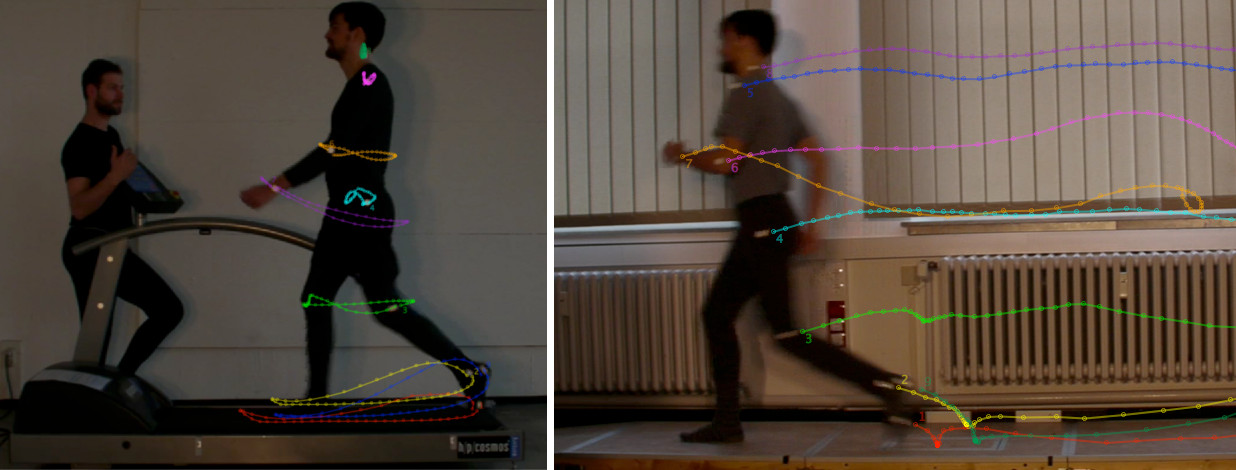
\includegraphics[width=\linewidth]{bilder/Einleitung/lauf_experimente.jpg}
	\caption[Experimente]{Links: Aufnahme aus dem Laufbandversuch mit getrackten Markern. Rechts: Aufnahme aus dem Laufstegversuch mit getrackten Markern.}
	\label{fig:experimente}
\end{figure}



%Der bipedale Gang des Menschen ist ein Erkennungsmerkmal unserer Fortbewegung und weist ein Alleinstellungsmerkmal gegenüber anderer bipedalen Bewegungsstilen auf: die fast vollständige Streckung der Beine (ALEXANDER 1992). Die Erforschung der menschlichen Fortbewegung erstreckt sich dabei von der Ganganalyse (alexander und wer noch so alles) über klinische Forschung (WREN ET AL 2011) bis hin zur Untersuchung von Laufmustern für Roboter (TLOK-XXX und ...noch eins..).
%Um den Gang genauer zu untersuchen wird der Gangzyklus grundlegend unterteilt in Standphase und Schwungphase sowie weitere Sub-Phasen, die in Abbildung \ref{fig:Skizze_Phasen} dargestellt sind (Perry XXX).\\
%Der Menschliche Gang lässt sich dabei sehr gut mit dem Modell eines inversen Pendels abstrahieren. Durch das fast vollständig gestreckte Standbein rotiert die Hüfte um den Kontaktpunkt mit dem Boden. Das Schwungbein verhält sich dagegen wie ein normales Pendel und schwingt um die Hüfte. Mit der Distanz des Beinschwerpunktes bis zur Hüfte lässt sich das Bein als mathematisches Pendel abstrahieren und so die Eigenfrequenz des Beines bestimmen. Bewegt man sich mit der Geschwindigkeit fort, bei der das jeweilige Schwungbein mit dieser Periodendauer schwingt, ist für die Beinbewegung keinerlei Energie notwendig (KUO 2007, HIER VLLT ANDERE QUELLE?!?!).\\

%Das Modell des inversen Pendels kann durch den subjektiven Energieaufwand beim Gehen überprüft werden. Bewegt man sich mit genau der richtigen Geschwindigkeit fort, sollte das Laufen als sehr angenehm empfunden werden und ohne großen Kraftaufwand möglich sein.
%\begin{wrapfigure}{r}{6cm}
%	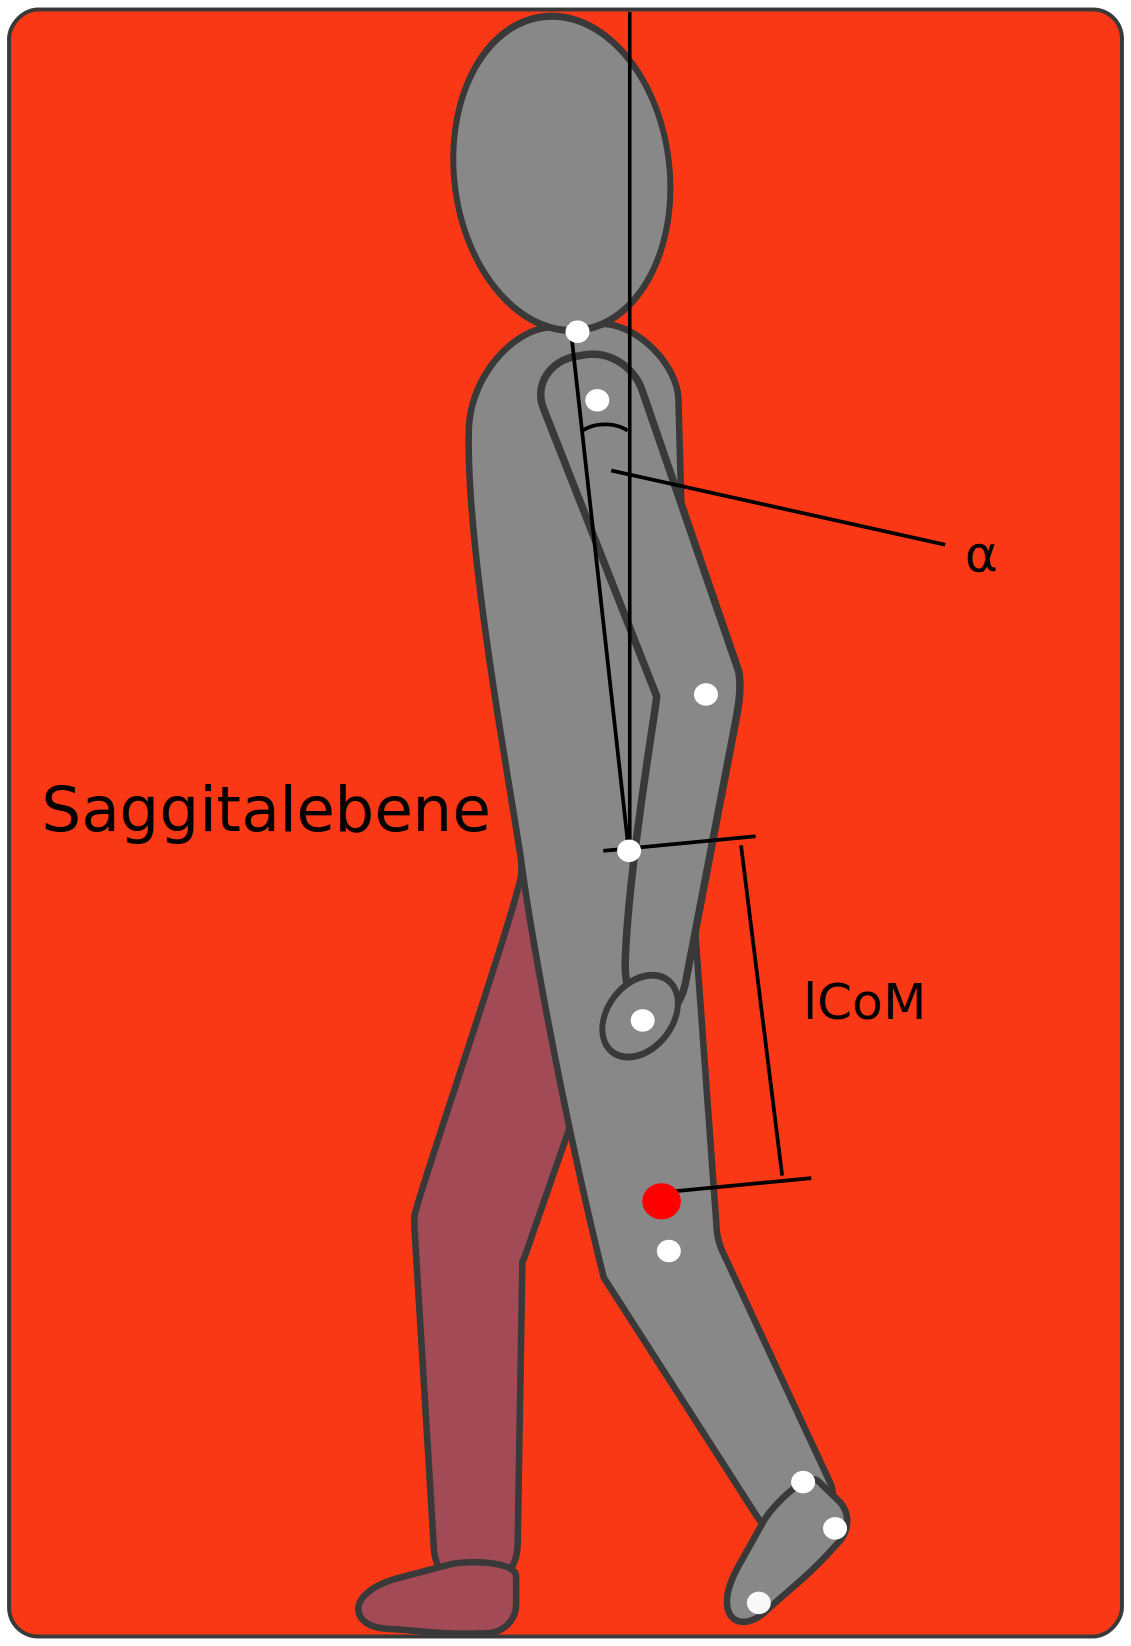
\includegraphics[width=\linewidth]{bilder/Einleitung/Proband_Pendel}
%	\caption[Inverses Pendel und untersuchte Gelenke]{Untersuchungsebene, wichtige Gelenke (weiße Kreise), Länge des virtuellen Pendels ($l_{CoM}$) von Hüfte bis zum Massenschwerpunkt des Beines (roter Kreis) sowie Neigungswinkel des Oberkörpers zur Senkrechten ($\alpha$)}
%	\label{fig:Proband_Pendel}
%\end{wrapfigure}
%Weitere Aussagen über den Gang lassen sich durch das Messen der Bodenreaktionskräfte (BRK) treffen. Verbindet man diese mit der kinematischen Analyse können Momente wie Lastaufnahme in Y-Richtung sowie ein Abbremsen und Abstoßen in X-Richtung beobachtet werden. Die Kräfte in Z-Richtung erlauben Aussagen über die Balance beim Gehen, welche besonders interessant sind für die monopedalen Stützphasen (ehhh, QUELLE?).
%Ziel dieser Arbeit ist die exemplarische Datenerhebung mittels kinematischer und kinetischer Verfahren für einen Probanden. Das Gehen wird bei verschiedenen Geschwindigkeiten untersucht und eine allgemeine Auswertung von Periodendauer durchgeführt, um die Theorie des inversen Pendels zu testen. Die Versuche auf dem Laufband und der Laufstrecke werden auf Unterschiede in der Körperneigung und der Handtrajektorie verglichen. Unterschiede zwischen den beiden Experimenten könnten auf eine Anpassung des Gehens an die tatsächliche Ortsänderung auf der Laufstrecke sein. Zusammen mit den Kraftmessungen werden mittels inverser Kinematik auf der Laufstrecke die auftretenden Kräfte und Momente in Knöchel, Knie und Hüfte untersucht und hier Aussagen zu ( JA ZU WAS DENN?? LAUFROBOTER??, BESSERE SCHUHE??) abgeleitet. Alle ermittelten Daten werden mit der Literatur verglichen und die Experimente auf ihre Belastbarkeit geprüft, da auf eine statistische Belastabrkeit der Messdaten verzichtet wurde, um den Umfang der Untersuchungen zu erhöhen.\\







%\begin{figure}
%	\centering
%	\includegraphics[width=0.7\linewidth]{bilder/Einleitung/gangphasen}
%	\caption[Gangphasen]{blabla blabla}
%	\label{fig:gangphasen}
%\end{figure}
\section{Material und Methoden}
%
%CALIBRIERUNG:
%LAsUFBAND 		   :	    245 pix = 1 m 
%LAUFSTRECKE		: 		260 pix = 1 m
%

\subsection{Proband}
Die Untersuchungen wurden an einer männlichen Person, 24 Jahre, 1,86\,m Körpergröße, 83\,kg Körpergewicht durchgeführt. Zum leichteren verfolgen der Gelenke wurden neun reflektierende Marker auf der linken Körperseite auf Ferse, Fußballen, Knöchel, Knie, Hüfte, Schulter, Hals, Ellenbogen und Handgelenk aufgebracht. Alle Laufversuche wurden ohne Schuhwerk, aber mit Socken durchgeführt.

\subsection{Laufband}
Die Laufbandversuche wurden durchgeführt auf einem mercury 4.0 Laufband (h/p/cosmos sports \& medical GmbH, Nussdorf-Traunstein, Deutschland). Videos wurden mit einer Samsung VP-HMX20C Videokamera (Samsung AG Seoul, Südkorea) mit einer Bildrate von 50~Hz, einer Belichtung von 1/1000~s und auf 5~m fixierten Fokus aufgenommen. 
Zur Ausleuchtung wurden zwei weißen 500W Baustrahlern aufgestellt. Abbildung~\ref{fig:laufbnd_stp} zeigt den Aufbau.\\
\begin{wrapfigure}{r}{6.5cm}
	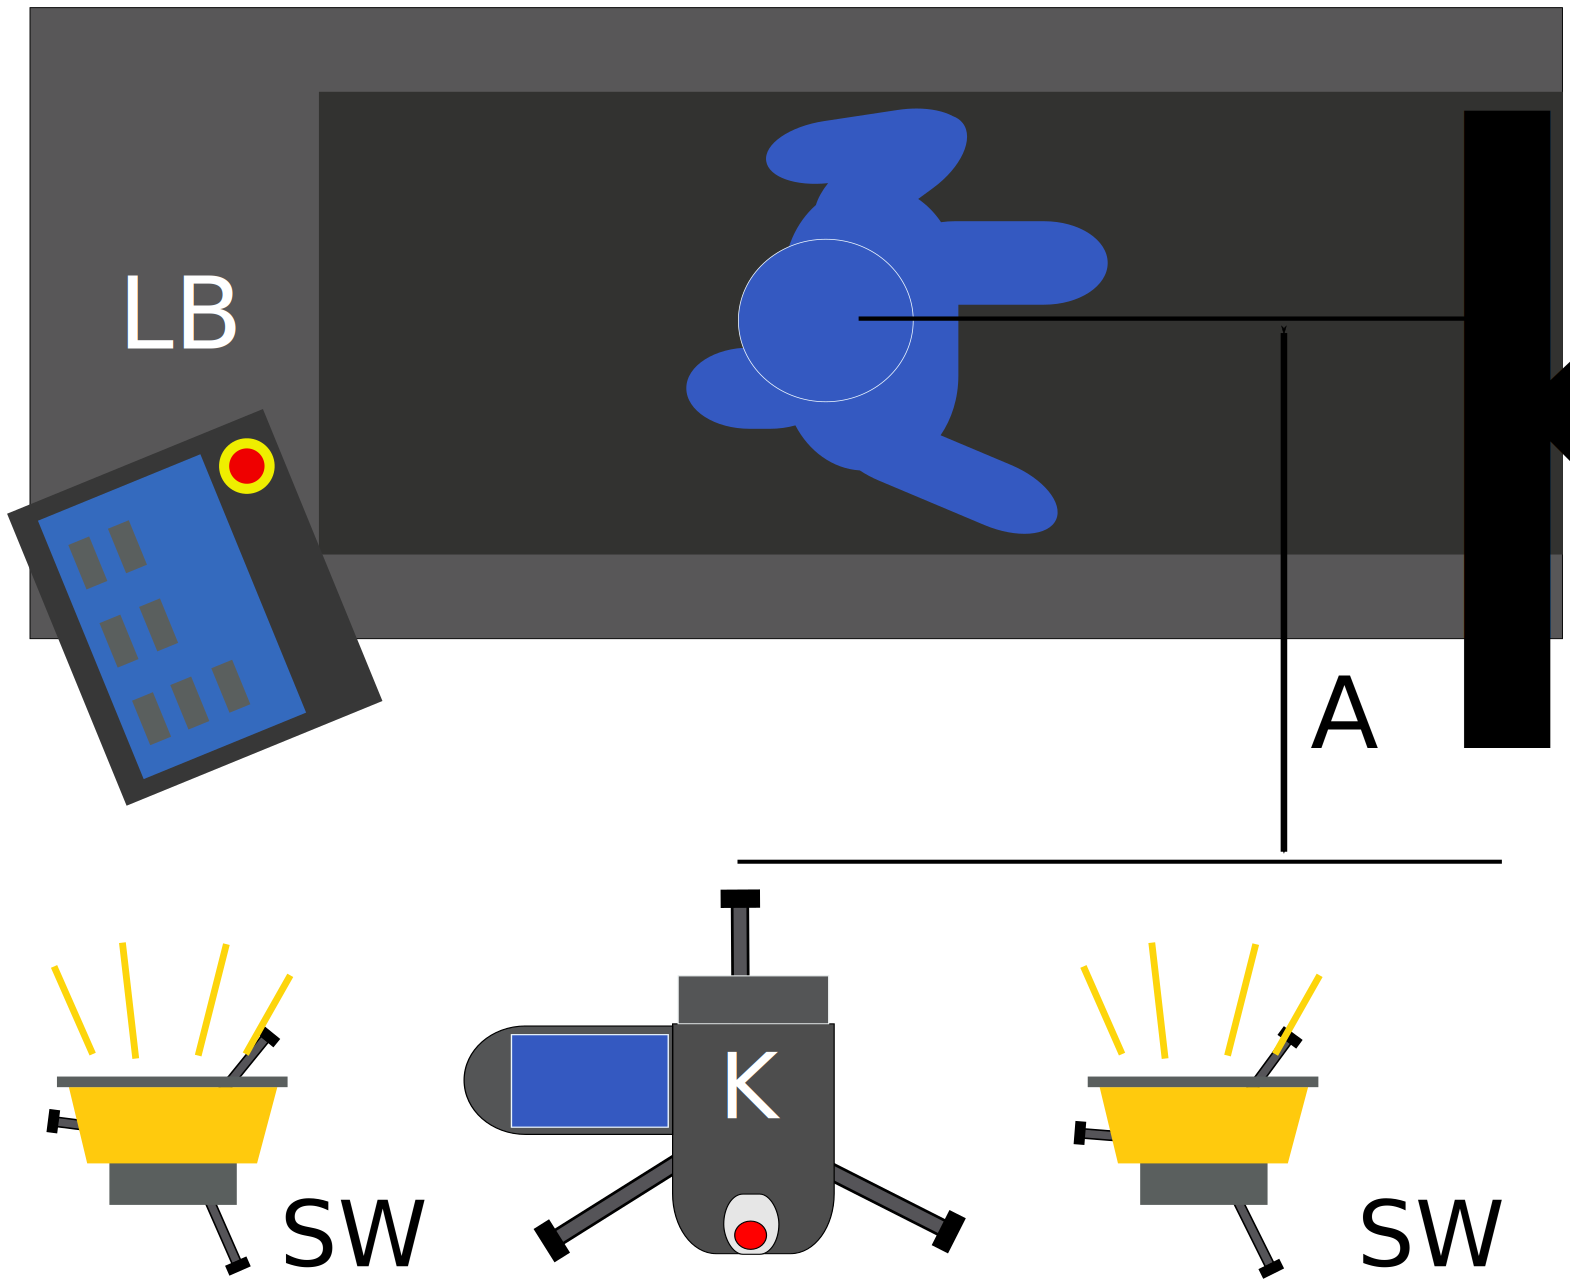
\includegraphics[width=\linewidth]{bilder/mat_met/Laufband_setup}
	\caption[Aufbau Laufband Versuch]{Aufbau des Laufband-Versuches mit Laufband LB, Kamera K und Scheinwerfern SW. Abstand zur Kamera $A_{Kam}$~=~5~m }
	\label{fig:laufbnd_stp}
\end{wrapfigure}

Es sollen sieben Gehgeschwindigkeiten untersucht werden. Hierfür wurden pro Geschwindigkeit jeweils mehrere Gangzyklen aufgenommen.\\
Bevor 
Nachdem sich der Proband an das Laufen auf dem Laufband gewöhnt hat, werden die Geschwindigkeiten von 1 bis 7\,km/h in 1\,km/h Schritten untersucht. Vor jeder neuen Videoaufnahme wird die Geschwindigkeit erhöht und der Proband hat Zeit, sich an die Geschwindigkeit anzupassen. Dabei wird auch eine subjektive Einschätzung verlangt, als wie anstrengend oder angenehm die aktuelle Laufgeschwindigkeit empfunden wird. Die subjektiven Einschätzungen werden nach Abschluss der Versuche in Werte von 1 (sehr unangenehm) bis 10 (sehr angenehm) überführt.\\

\subsection{Laufstrecke mit Kraftmessplatte}
Für die Versuche auf der Laufstrecke soll der Proband in drei Geschwindigkeiten, welche als {langsam}, angenehm und schnell eingeschätzt werden, über die Laufstrecke gehen und dabei auf der Waage mit seinem linken Fuß möglichst zentral auftreten.\\
Videokamera und Baustrahler des Laufband-Versuches kommen auch hier zum Einsatz. Die Laufstrecke ist ein Eigenbau der Hochschule Bremen. Ein Quarzkristall-3-Komponenten-Dynanometer Typ 9257B (Kistler Gruppe Winterthur, Schweiz), im Folgenden {Waage} genannt, wird unter einer Platte (\textbf{ABMESSUNGEN}) eingebaut. Die Waage ist über einen Mehrkanal-Ladungsverstärker Typ 5070A (Kistler) mit einem Computer verbunden. Abbildung~\ref{fig:laufstg_stp} zeigt den Aufbau. Die Kamera steht zentriert vor der Waage und die Bildebene ist parallel zur Saggitalebene ausgerichtet.
Das Waagenzentrum liegt in den Aufnahmen bei x = 1.554\,m, y = 0.099\,m von der linken unteren Bildecke aus.
\begin{figure}[h!]
	\centering
	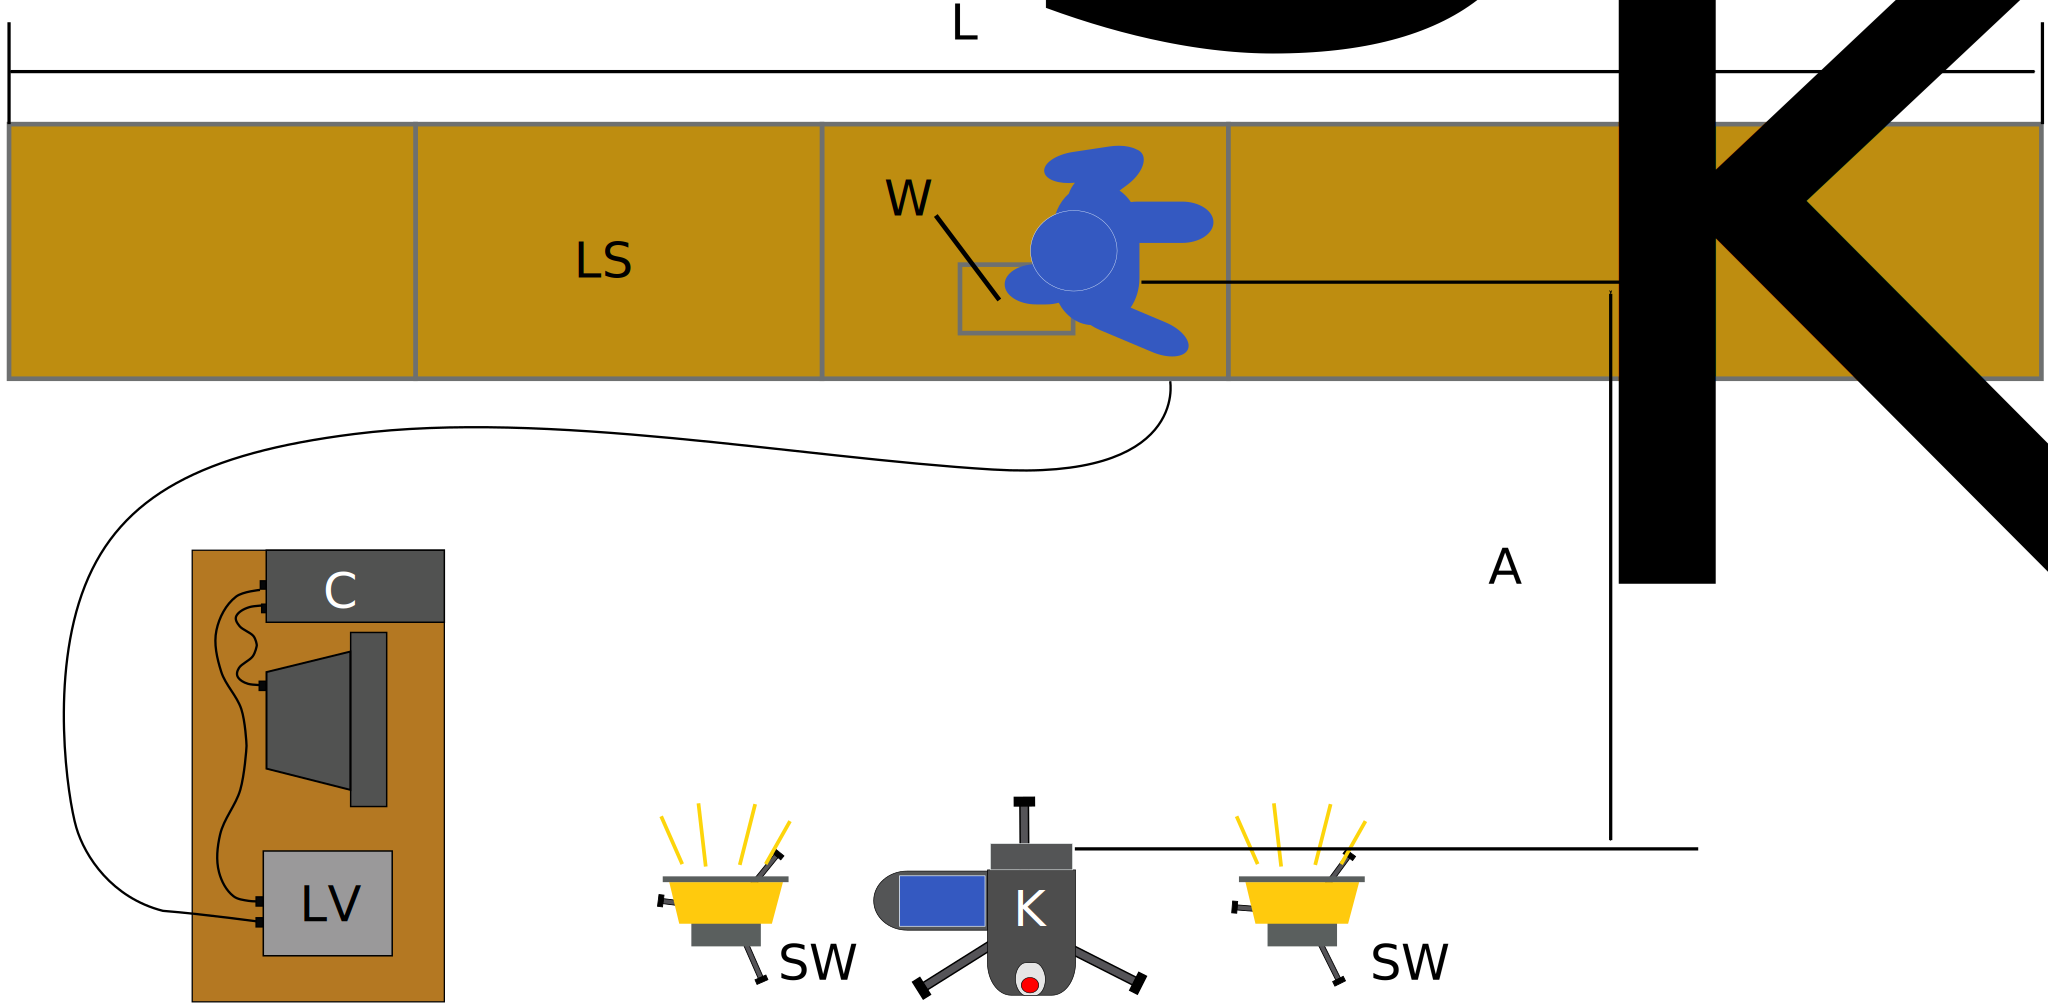
\includegraphics[width=0.7\linewidth]{bilder/mat_met/Laufstrecke_setup}
	\caption[Aufbau Laufstrecke Versuch]{Aufbau des Laufstrecke-Versuches mit Laufstrecke LS, Kamera K, Scheinwerfern SW, Computer C, Waage W und Ladungsverstärker LV. Länge Steg $L_S~=~6~m$ und Abstand zur Kamera $A_{Kam}~=~5~m$}
	\label{fig:laufstg_stp}
\end{figure}

Die Kameraeinstellungen vom Laufbandversuch übernommen finden auch hier Anwendung. Die Digitalisierung der Koordinaten ist wie oben beschrieben durchgeführt worden. Die Waagensignale werden mit 100\,Hz und 200\,N/V vom Ladungsverstärker an den Computer weitergeleitet. Mit DASYLab (Measurement Computing, Norton, USA) werden die Eingangssignale verarbeitet und alle 8 Kanäle im ASCII-Format gespeichert.
Für eine 4-Punkt-Kalibration wird die Waage in alle drei Raumrichtungen mit 0, 1, 3,6 und 7,75\,kg belastet. Der Waagendrift wird über 30\,s ohne Belastung für jede Raumrichtung ermittelt.\\
Das Gehen über die Waage muss einige Male geübt werden, so dass die Waage mit dem Linken Fuß möglichst zentral belastet wird, dies aber nicht durch eine Änderung des Ganges erreicht wird. 

\subsection{Datenauswertung}
Alle verwendeten Videos werden mit dem Programm ffmpeg 2.1 (LGP License, ffmpeg.org) in Einzelbilder zerlegt. Es wird für jeden Versuch eine Bildsequenz ausgewählt, welche einem Schritt (linkes Bein abheben, schwingen, aufsetzen, belasten und entlasten) entspricht. Das Programm ImageJ (National Institutes of Health Bethesda, Maryland) mit dem Plugins MTrackJ \textbf{CITE(Meijering 20120)} erlaubt dann das Erfassen der xy-Koordinaten der Gelenke in jedem Einzelbild. Für die sieben ausgewählten Bildsequenzen des Laufbandexperiments und die drei Sequenzen des Laufstreckenexperiments werden jeweils neun Marker verfolgt und der Datensatz im .mdf-Format gespeichert.
Die Dauer der Schwungphase, der Standphase und des gesamten Schrittzyklus sowie der Duty-Faktor werden aus den Bildsequenzen bestimmt. Der Dutyfaktor ist wie folgt definiert:
\begin{equation}
\mathrm{DF} = \frac{\mathrm{T_{Stand}}}{\mathrm{T_{Schritt}}}
\end{equation}
Die weitere Auswertung der erhaltenen Trajektorien und Waagenausgabe erfolgt in der Skriptsprache Scilab (Scilab Enterprises S.A.S., Orsay Cedex, France). Im folgenden sollen die verwendeten Algorithmen beschrieben werden, für die  genaue Implementierung sei auf den Quellquode auf der beigefügte CD.\\
\subsubsection{Datenstruktur}
In einem objektorientierten Ansatz werden Strukturen geschaffen, welche ein möglichst gut verständliches Abbild der physikalisch-biologischen Beschreibung bieten. Dies wird erreicht durch eine Schachelung von Containern und Eigenschaften. Der Datensatz eines Experiments wird so zusammengefasst in einem 'Körper', der Körper beinhaltet nun alle Gelenke und Körpersegmente, welche wiederum ihre Eigenschaften wie Masse und Trägheitsradius, sowie den zeitlichen Verlauf von Ort, Geschwindigkeit, Winkel etc. beinhalten. 
\subsubsection{Numerische Verfahren}
Die Geschwindigkeit eines Punktes ergibt sich aus der zeitlichen Ableitung seines Ortes. Die Bestimmung der Geschwindigkeit v zum Zeitpunkt t aus diskreten Ortswerten $\mathrm{x(t - \Delta{t})}$ und $\mathrm{x(t + \Delta{t})}$wird durch die Verwendung der Zentraldifferenz durchgeführt:
\begin{equation}
	\vec{v}(t) = \frac{\vec{x}(t + \Delta{t}) - \vec{x}(t - \Delta{t})}{2\Delta{t}}
\end{equation}
Für die Randwerte, d.h. den ersten und letzten Mittelwert, wird mangels Stützstellen eine Vorwärts-, beziehungsweise Rückwärtsdifferenz durchgeführt.
Abgeleitete Daten wie Geschwindigkeit, Beschleunigung und Winkel, sowie die Kraftwerte werden durch einen gleitenden Mittelwert geglättet:
\begin{equation}
	    \vec{\phi}(t) = \frac{a\,\phi(t - \Delta{t}) + b\,\phi(t) + c\,\phi(t - \Delta{t})}{a + b + c}
\end{equation}
Werden die Gewichtungsfaktoren a, b und c auf 1 gesetzt, erhält man einen gleitenden Mittelwert mit drei Stützstellen. Ein Ändern der Gewichtungsfaktoren erzeugt einen gewichteten Mittelwert. Die Randwerte werden hierbei nicht geglättet.\\
Der Winkel zwischen zwei Gelenken wird durch triviale Trigonometrie berechnet und ist in den Ergebnissen, falls keine weitere Erläuterung vorhanden ist, jeweils im mathematischen Sinne und in Grad angegeben. 

\subsubsection{Anthropometrie}
Mit Hilfe der Tabelle \textbf{NEED TABELLE} können die Eigenschaften eines Segmentes aus dem Körpergewicht, sowie den Ortsvektoren von den benachbarten Gelenken bestimmt werden. CoM (center of mass) steht für den Masseschwerpunkt, d für das distale Gelenk und p für das proximale Gelenk. Der Ortsvektor des Masseschwerpunktes eines Segmentes wird mit Hilfe eines Faktors $c_{seg}$ aus der Antropometrietabelle berechnet:
\begin{equation}
\vec{x}_{CoM} = (\vec{x}_d - \vec{x}_p) \cdot c_{seg} + \vec{x}_p
\label{eq:CoM_x}
\end{equation}

\subsection{Auswertung Laufband}
Die Frequenz des Beinschwingens wird mit der Frequenz eines mathematischen Pendels verglichen. Die Frequenz des Schwingens ergibt sich aus der Zeit zwischen Abheben und Aufsetzen eines Fußes. Die Frequenz ist der Kehrwert der Periodendauer, eine Periode bezeichnet das Hin- und Zurückschwingen des Pendels, weshalb $\mathrm{T_{Schwung}}$ mit zwei multipliziert wird:
\begin{equation}
\mathrm{f_{Schwung}} = 1 / (2 * (\mathrm{T_{Schwung}}))
\end{equation}
Die Periodendauer T eines mathematischen Pendels (konstante Länge L zwischen Aufhängung und Punktmasse) ergibt sich aus:
\begin{equation}
	T = 2  \pi \sqrt{\frac{L}{g}} 
\end{equation}
Diese Gleichung gilt für kleine Auslenkungswinkel ($\le$ 5 Grad). Die Pendellänge L wird bestimmt als der Abstand zwischen der Aufhängung Hüfte und des Masseschwerpunktes des gesamten Beines.
Als Vergleich und Validierung wird die eingestellte Laufbandgeschwindigkeit zwei Berechnungsmethoden gegenübergestellt. Die Geschwindigkeit lässt sich aus den Videodateien als diejenige definieren, mit der sich der Fuß fortbewegt, wenn er fest auf dem Band steht. Weiterhin kann die Fortbewegungsgeschwindigkeit des Probanden relativ zum Laufband aus der doppelten Schrittfrequenz und der Schrittweite pro Schritt bestimmt werden.
\begin{equation}
v_{\mathrm{calc}} = f_{\mathrm{fSchritt}} \cdot 2 \cdot x_{\mathrm{Schritt}} \cdot 3,6\;\frac{\mathrm{km/h}}{\mathrm{m/s}}
\end{equation}

\subsubsection{Inverse Dynamik}
Die inverse Dynamik erlaubt die Bestimmung von Kraft und Momenten in Gelenken, ohne Messungen an den jeweiligen Gelenken durchführen zu müssen. Hierfür werden die Segmente zwischen zwei Gelenken als Balkenelemente abstrahiert und die Gelenke als einfache Lager. Durch Aufstellen von Kraft- und Momentengleichgewichten können, ausgehend von der auf die Waage wirkenden Kräfte in Knöchel, Knie und Hüfte bestimmt werden. Die aufgestellten Gleichungen sind im Anhang zu finden.

\subsubsection{Vergleich Laufband - Laufstrecke}
Die Neigung des Oberkörpers wird durch den Winkel, welcher zwischen der Verbindung von Hüfte zu Nacken und der x Koordinate anliegt. Ein Winkel von 0 Grad entspricht dabei einem aufrechten Oberkörper, postive Winkel einer Vorbeugung, negative Winkel zeigen einen nach hinten gebeugten Oberkörper an. \\
Um die Trajektorien der Hände vergleichbar machen zu können, wird der Ortsvektor des Handgelenks relativ zum Nacken dargestellt. 







\section{Ergebnisse}
\subsection{Laufband}
In \autoref{tab:laufband} sind die eingestellten, ermittelten und berechneten Parameter für die verschiedenen Gangstile des Laufbandexperiments aufgetragen. Der Duty-Faktor beschreibt das Verhältnis von Auftrittsdauer zu Schrittdauer. Er sinkt mit zunehmender Geschwindigkeit ab, bleibt jedoch für alle Geschwindigkeiten über dem kritischen Wert von 0,5. Die Schwungfrequenz steigt nur leicht mit zunehmender Geschwindigkeit, die Schrittfrequenz verdoppelt sich von der geringsten zur höchsten Ganggeschwindigkeit. \\
Aus allen Messreihen (10 Stück) ergibt sich ein durchschnittlicher Wert für die Länge des Bein-Pendels (Abstand Hüfte - Schwerpunkt gesamtes Bein) von 0.37\,m, es ergibt sich hieraus eine Periodendauer von 1,22\,s beziehungsweise eine Frequenz von 0,82\,Hz für den Schwungvorgang. \\
Weiterhin wird ein Vergleich mit dem inversen Pendel-Modell angestrebt. Als Pendellänge wird hierzu die Beinlänge gewählt, welche als 0,94\,m bestimmt wurde. Es ergibt sich dann eine Periodendauer von 1,94\,s. Die Periodendauer der Standphase, also jener Zeit in der die Hüfte um den Standmittelpunkt pendelt, ergibt sich aus der doppelten Dauer einer Standphase. \\

\begin{table}[h!]
	\centering
	\caption[Abgeleitete Größen]{Übersicht der Laufparameter bei den sieben verschiedenen Gehgeschwindigkeiten, welche auf dem Laufband untersucht wurden. Die errechnete Geschwindigkeit wird aus Schrittfrequenz und -weite bestimmt, die gemessene Geschwindigkeit entspricht der Horizontalgeschwindigkeit des Fußes beim Stillstand auf dem Laufband. Die Standperiode wird mit einem Inversen Pendel mit Pendellänge 0,94\,m verglichen. Die subjektive Bewertung geht von 1 (sehr unangenehm) bis 10 (sehr angenehm);}
	\label{tab:laufband}
	\begin{tabular}{L{5.5cm}C{0.9cm}C{0.9cm}C{0.9cm}C{0.9cm}C{0.9cm}C{0.9cm}C{0.9cm}}
		\toprule
		\textbf{Eingestellte Geschw. [kmh]} & 1.00 & 2.00 & 3.00 & 4.00 & 5.00 & 6.00 & 7.00\\
		\midrule 
		\textbf{Duty-Faktor} 		& 0.78 & 0.71 & 0.68 & 0.66 & 0.60 & 0.59 & 0.58 \\
		\textbf{Schwungfrequenz [Hz]} & 1.09 & 1.14 & 1.14 & 1.25 & 1.14 & 1.25 & 1.25 \\
		\textbf{Schrittfrequenz [Hz]} & 0.47 & 0.66 & 0.72 & 0.86 & 0.90 & 1.02 & 1.04 \\
		\textbf{Schrittweite [m] }& 0.37 & 0.50 & 0.69 & 0.75 & 0.85 & 0.88 & 0.97 \\
		\midrule
		\textbf{Errechnete Geschw. [kmh]} & 1.25 & 2.37 & 3.56 & 4.65 & 5.51 & 6.44 & 7.19 \\
		\textbf{Gemessene Geschw. [kmh]} & 0.93 & 1.93 & 3.09 & 4.16 & 5.02 & 6.27 & 7.15 \\
		\midrule
		\textbf{Subj. Bewertung } & 1 & 3 & 6 & 7 & 10 & 6 & 4 \\
		 \textbf{Periode Stand [s]} &  3.32 &  2.15 &  1.89 & 1.53 &  1.33 &  1.15 & 1.12 \\
		\textbf{Abweichung Pendel [\%]}  & +71 & +11 & -3 & -21 & -31 & -41 & -43 \\
%		& 33 & 39 & 39 & 52 & 39 & 52 & 52 \\
		\bottomrule
	\end{tabular}
\end{table}

Im letzten Abschnitt der Tabelle ist der Vergleich der Gangarten mit dem inversen Pendel Modell aufgetragen.\\ 
Es ergibt sich eine minimale Abweichung der Periodendauer von 3\,\%{} für eine Geschwindigkeit für 3\,\kmh. Für langsamere Geschwindigkeiten steigt die Standdauer, bei höheren Geschwindigkeiten sinkt sie. Die als subjektiv am angenehmsten Empfundene Geschwindigkeit ist 5\,\kmh. Am wenigsten angenehm empfunden wurde eine Gehgeschwindigkeit von 1\,\kmh. 

\subsection{Laufstrecke}
Auf der Laufstrecke wurden drei Durchgänge mit vom Probanden als langsam, angenehm und schnell empfundenen Geschwindigkeiten durchgeführt. Eine Übersicht über die verschiedenen Gangstile findet sich in \autoref{tab:laufstrecke}. 
Die Schwungfrequenz steigt mit zunehmender Geschwindigkeit an. Die Schrittfrequenz unterscheidet steigt von 0,93 bei 1,61\,\kmh auf 1,39 bei 8,58\,\kmh um 178\,\% an. 

 \begin{table}[h!]
	\centering
	\caption[Übersicht Laufstrecke]{Parameter der drei gewählten Gehgeschwindigkeiten des Laufstreckenversuchs. Die Geschwindigkeit des Nackens bezieht sich auf die berechnete durchschnittliche Horizontalgeschwindigkeit des Nackenmarkers.}
	\label{tab:laufstrecke}
	\begin{tabular}{L{4.5cm}C{1.5cm}C{2cm}C{2cm}C{2cm}}
		\toprule
		\textbf{Geschw. gefühlt}& langsam & angenehm & schnell \\
		\midrule
		\textbf{Duty-Faktor}	& 0.75 & 0.64 & 0.53 \\
		\textbf{Schwungfrequenz [Hz]} & 0.93 & 1.19 & 1.39 \\
		\textbf{Schrittfrequenz [Hz]} & 0.46 & 0.86 & 1.28 \\
		\textbf{Geschw. Nacken [kmh]}& 1.61 & 4.45 & 8.58 \\
		\bottomrule
		
	\end{tabular}
\end{table}

\subsubsection{Bodenreaktionskräfte}
Die Kräfte, welche von der Waage aufgenommen und in Newton umgerechnet wurden, sind für die drei untersuchten Geschwindigkeiten in \autoref{fig:grf} über den entdimensionierten Schrittzyklus aufgetragen. Die Kräfte wurden nur für die Standphase aufgetragen.\\
Die Bodenreaktionskraft des langsamen Gehens (rote Kurve) beginnt mit einer zunächst kleinen Belastung, welche nach einem kurzen Plateau nahezu linear ansteigt und ein zweites Plateau erreicht und danach wiederum auf 0 absinkt. Das zweite Plateau markiert das Stehen auf einem Bein und dauert etwa 35\,\% des gesamten Schrittzykluses an. Die Bodenreaktionskraft überschreitet zu keinem Zeitpunkt die Gewichtskraft des Probanden.\\

\begin{figure}[h!]
	\centering
	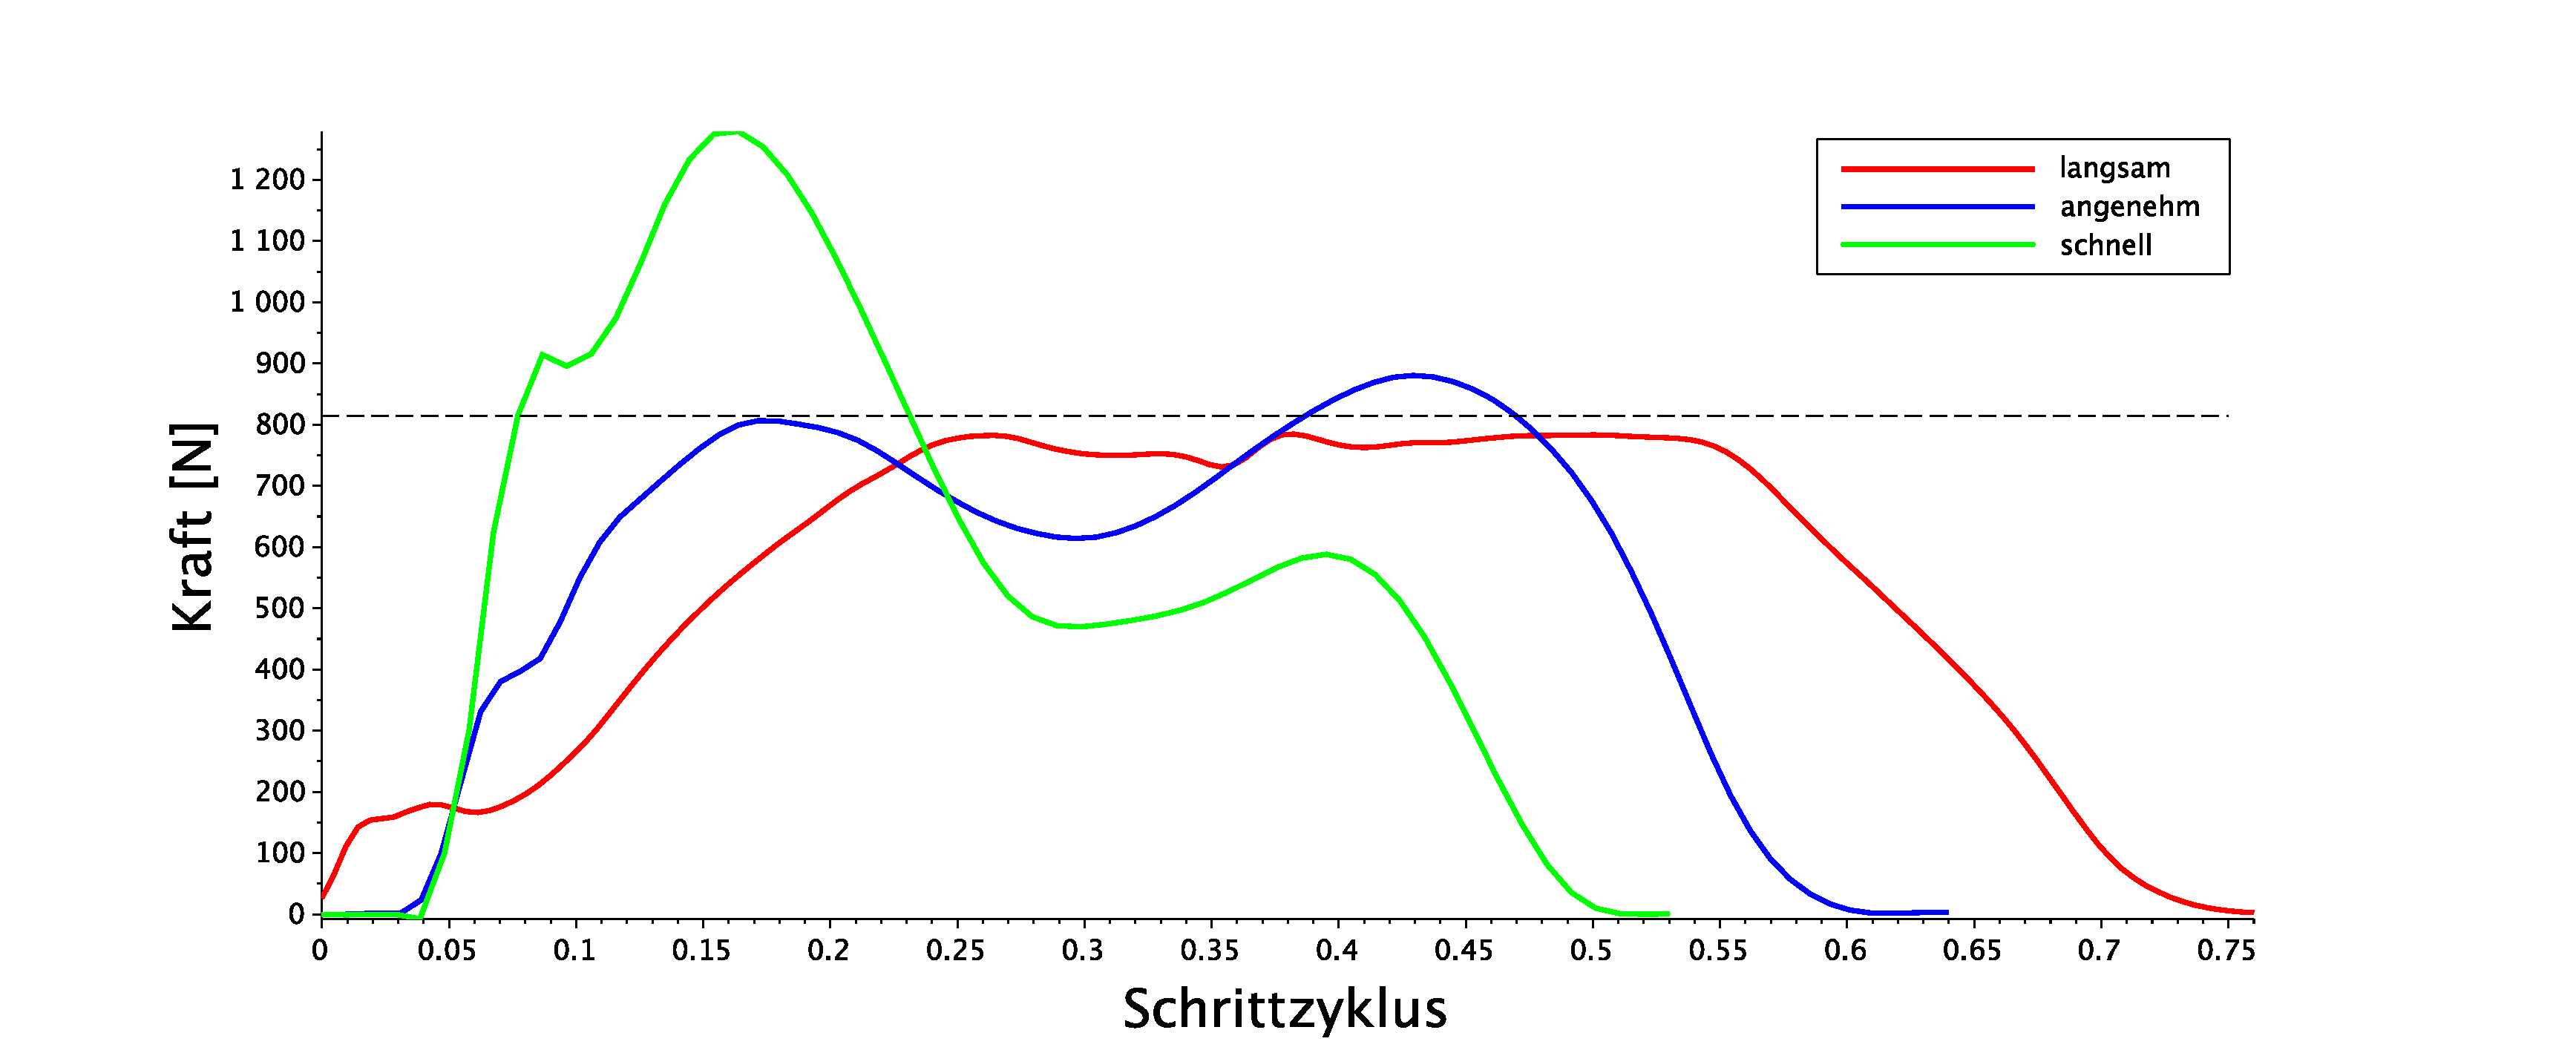
\includegraphics[width=1\linewidth]{bilder/ergebnisse/Forces_df_plusbw.pdf}
	\caption[Bodenreaktionskräfte]{Verlauf der Bodenreaktionskräfte entgegen der Gravitationsrichtung über den entdimensionierten Schrittzyklus. Schwarz gestrichelte Linie: Gewichtskraft des Probanden.}
	\label{fig:grf}
\end{figure}

Das angenehme Gehen (blaue Kurve) ist durch drei charakteristische Höcker gekennzeichnet. Direkt nach Beginn der Belastung zeigt sich ein kleinerer Knick, woraufhin die Belastung weiter ansteigt und den Wert der Gewichtskraft erreicht. Die Belastung sinkt daraufhin auf ein lokales Minimum von 609\,N ab, was 75\,\% der Gewichtskraft entspricht. Im weiteren Verlauf steigt die Bodenreaktionskraft erneut an auf 880\,N beziehungsweise 108\,\% der Gewichtskraft. \\
Die Kräfte des schnellen Gehens sind in grün eingezeichnet. Sie steigen zunächst stark an und weisen einen ersten Knick bei 905\,N auf. Das im weiteren Verlauf erreichte Maximum von 1275\,N (156\,\% Gewichtskraft) wird nach etwa einem fünftel der Standdauer erreicht. Die Bodenreaktionskraft sinkt daraufhin ab und erreicht ein weiteres Plateau und ein lokales Maximum von 582\,N, bevor sie auf null absinkt.\\

\subsubsection{Inverse Dynamik}
Neben den in \autoref{fig:grf} aufgetragenen vertikalen Kräften wurden zudem die Kräfte in Laufrichtung und quer zur Laufrichtung aufgenommen. Über die inverse Dynamik lassen sich so die Kräfte in den Gelenken berechnen.
In \autoref{fig:knee_forces} sind für das Knie die Kräfte in Laufrichtung (Fx), entgegen der Gravitation (Fy) und das Moment um die Achse senkrecht zur Bildebene für die angenehme Geschwindigkeit aufgetragen. Die Kräfte sind hier nur für die Dauer der Standphase eingezeichnet. Der Verlauf von Fy (blau) ist von zwei Höckern gezeichnet, weist im Vergleich zu den Bodenreaktionskräften jedoch keinen anfänglichen Knick auf. Die in rot eingetragenen Kräfte in Laufrichtung (Fx), sind zunächst negativ, nach etwas mehr als der Hälfte der Belastungsdauer wechseln sie ins positive mit einem maximalen Wert von 112\,N. 
\textbf{DAS DUMME MOMENT MACHT NICHT WAS ES SOLL?}
\begin{figure}[h!]
	\centering
	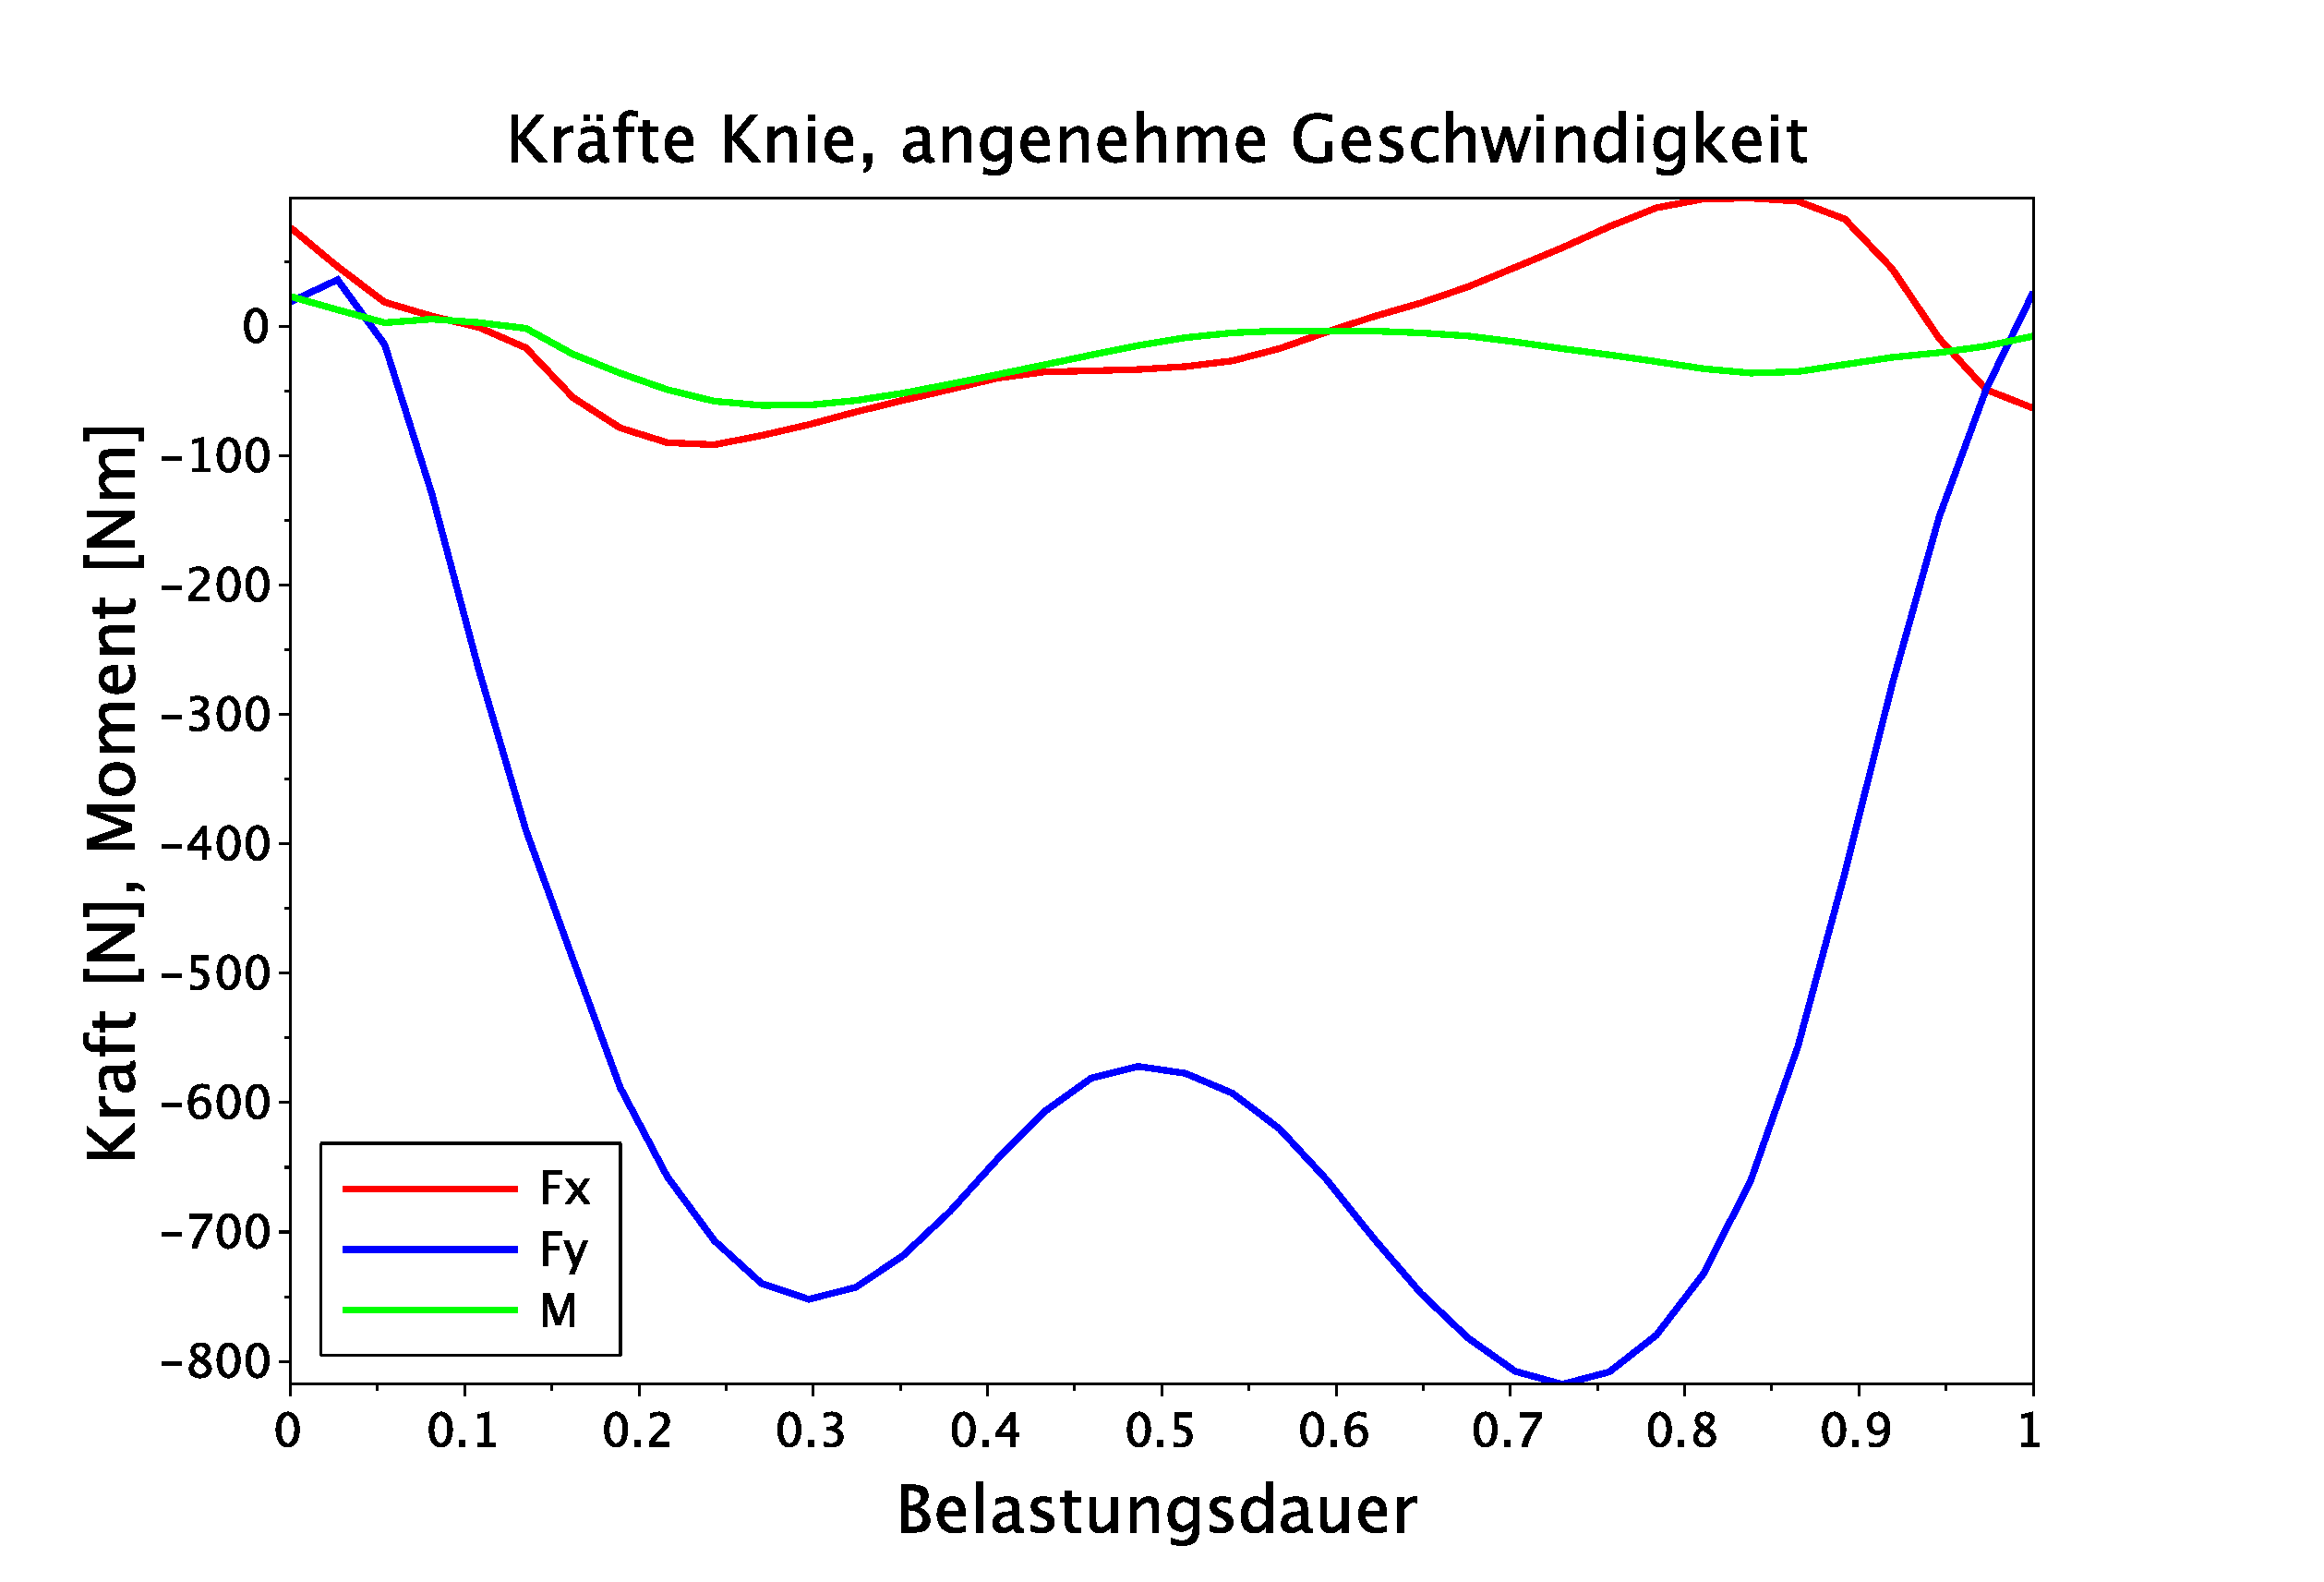
\includegraphics[width=0.7\linewidth]{bilder/ergebnisse/forces_knee.pdf}
	\caption[Bodenreaktionskräfte]{Verlauf von $F_x$, $F_y$ und $M$ während der Standphase.}
	\label{fig:knee_forces}
\end{figure}

Für einen Vergleich der bei verschiedenen Geschwindigkeiten wirkenden Kräfte sind in \autoref{fig:ankle_fx} die Laufrichtung wirkenden Kräfte (Fx) geplottet. Für eine bessere Vergleichbarkeit wurden alle Geschwindigkeiten auf eine gemeinsame x-Achse, der entdimensionierten Belastungsdauer, aufgetragen. Allen Kurven ist gemein, dass sie im positiven starten, ins negative abfallen und nach etwa der halbe Belastungsdauer ins positive Wechseln. Die Kraftverläufe sind dabei annähernd punktsymmetrisch zum Nulldurchgang. Die beim langsamen Gehen auftretenden Kräfte sind kleiner als die der höheren Geschwindigkeiten. Die größte negative Kraft beträgt -32\,N, die größte positive Kraft beträgt 59\,N. \\
Das angenehme Gehen (blau) weist einen ähnlichen Verlauf, mit größeren Extremwerten von -109 und 124\,N. Die Kräfte, welche beim schnellen Gehen auftreten sind noch größer, mit -163 und 132\,N. Im Gegensatz zu den langsameren Geschwindigkeiten ist hier der Betrag des negativen Extremwertes größer als der des später auftretenden positiven Extremwertes.\\
\begin{figure}[h!]
	\centering
	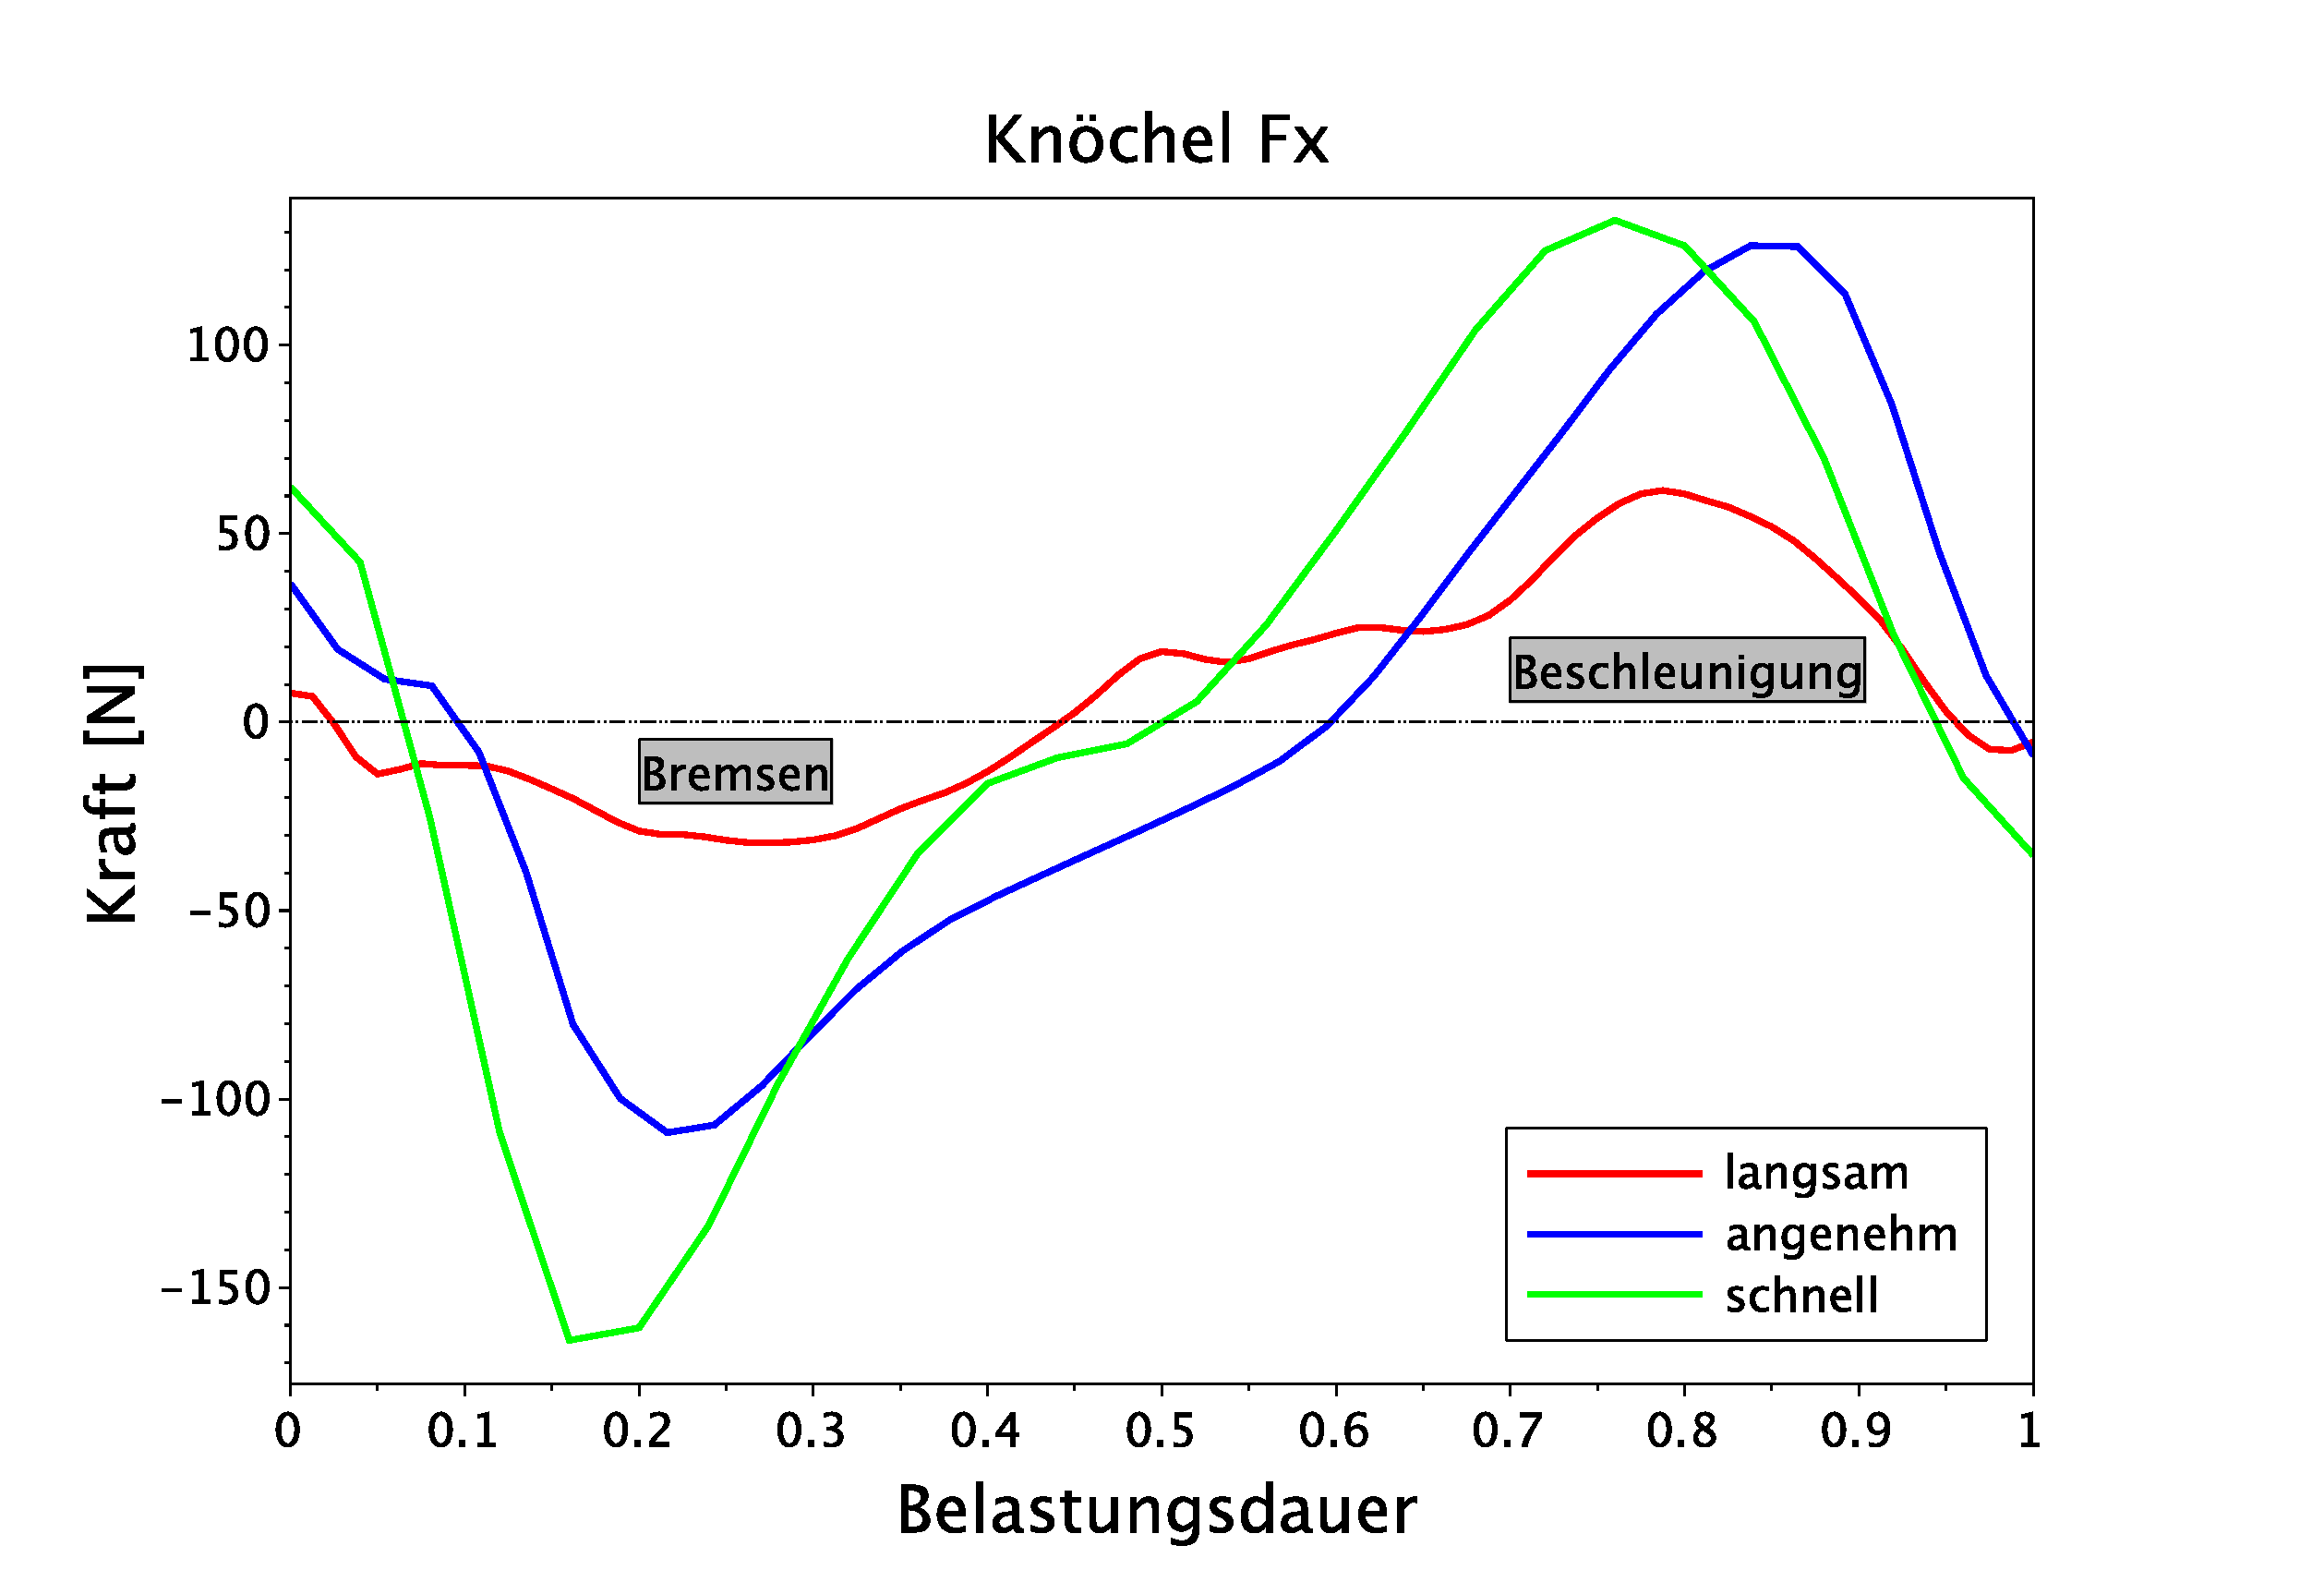
\includegraphics[width=0.7\linewidth]{bilder/ergebnisse/ankle_fx_plot.pdf}
	\caption[Bodenreaktionskräfte]{Verlauf von $F_x$ im Knöchel während der Standphase. Negative Kräfte treten zu Beginn der Standphase auf, Ab der mittleren Standphase treten positive Kräfte auf.}
	\label{fig:ankle_fx}
\end{figure}

Aus sportmedizinischer Sicht interessant sind die bei der Lokomotion auftretenden Momente im verletzungsanfälligen Knie, welche in \autoref{fig:knee_m} eingezeichnet sind. 

\begin{figure}[h!]
	\centering
	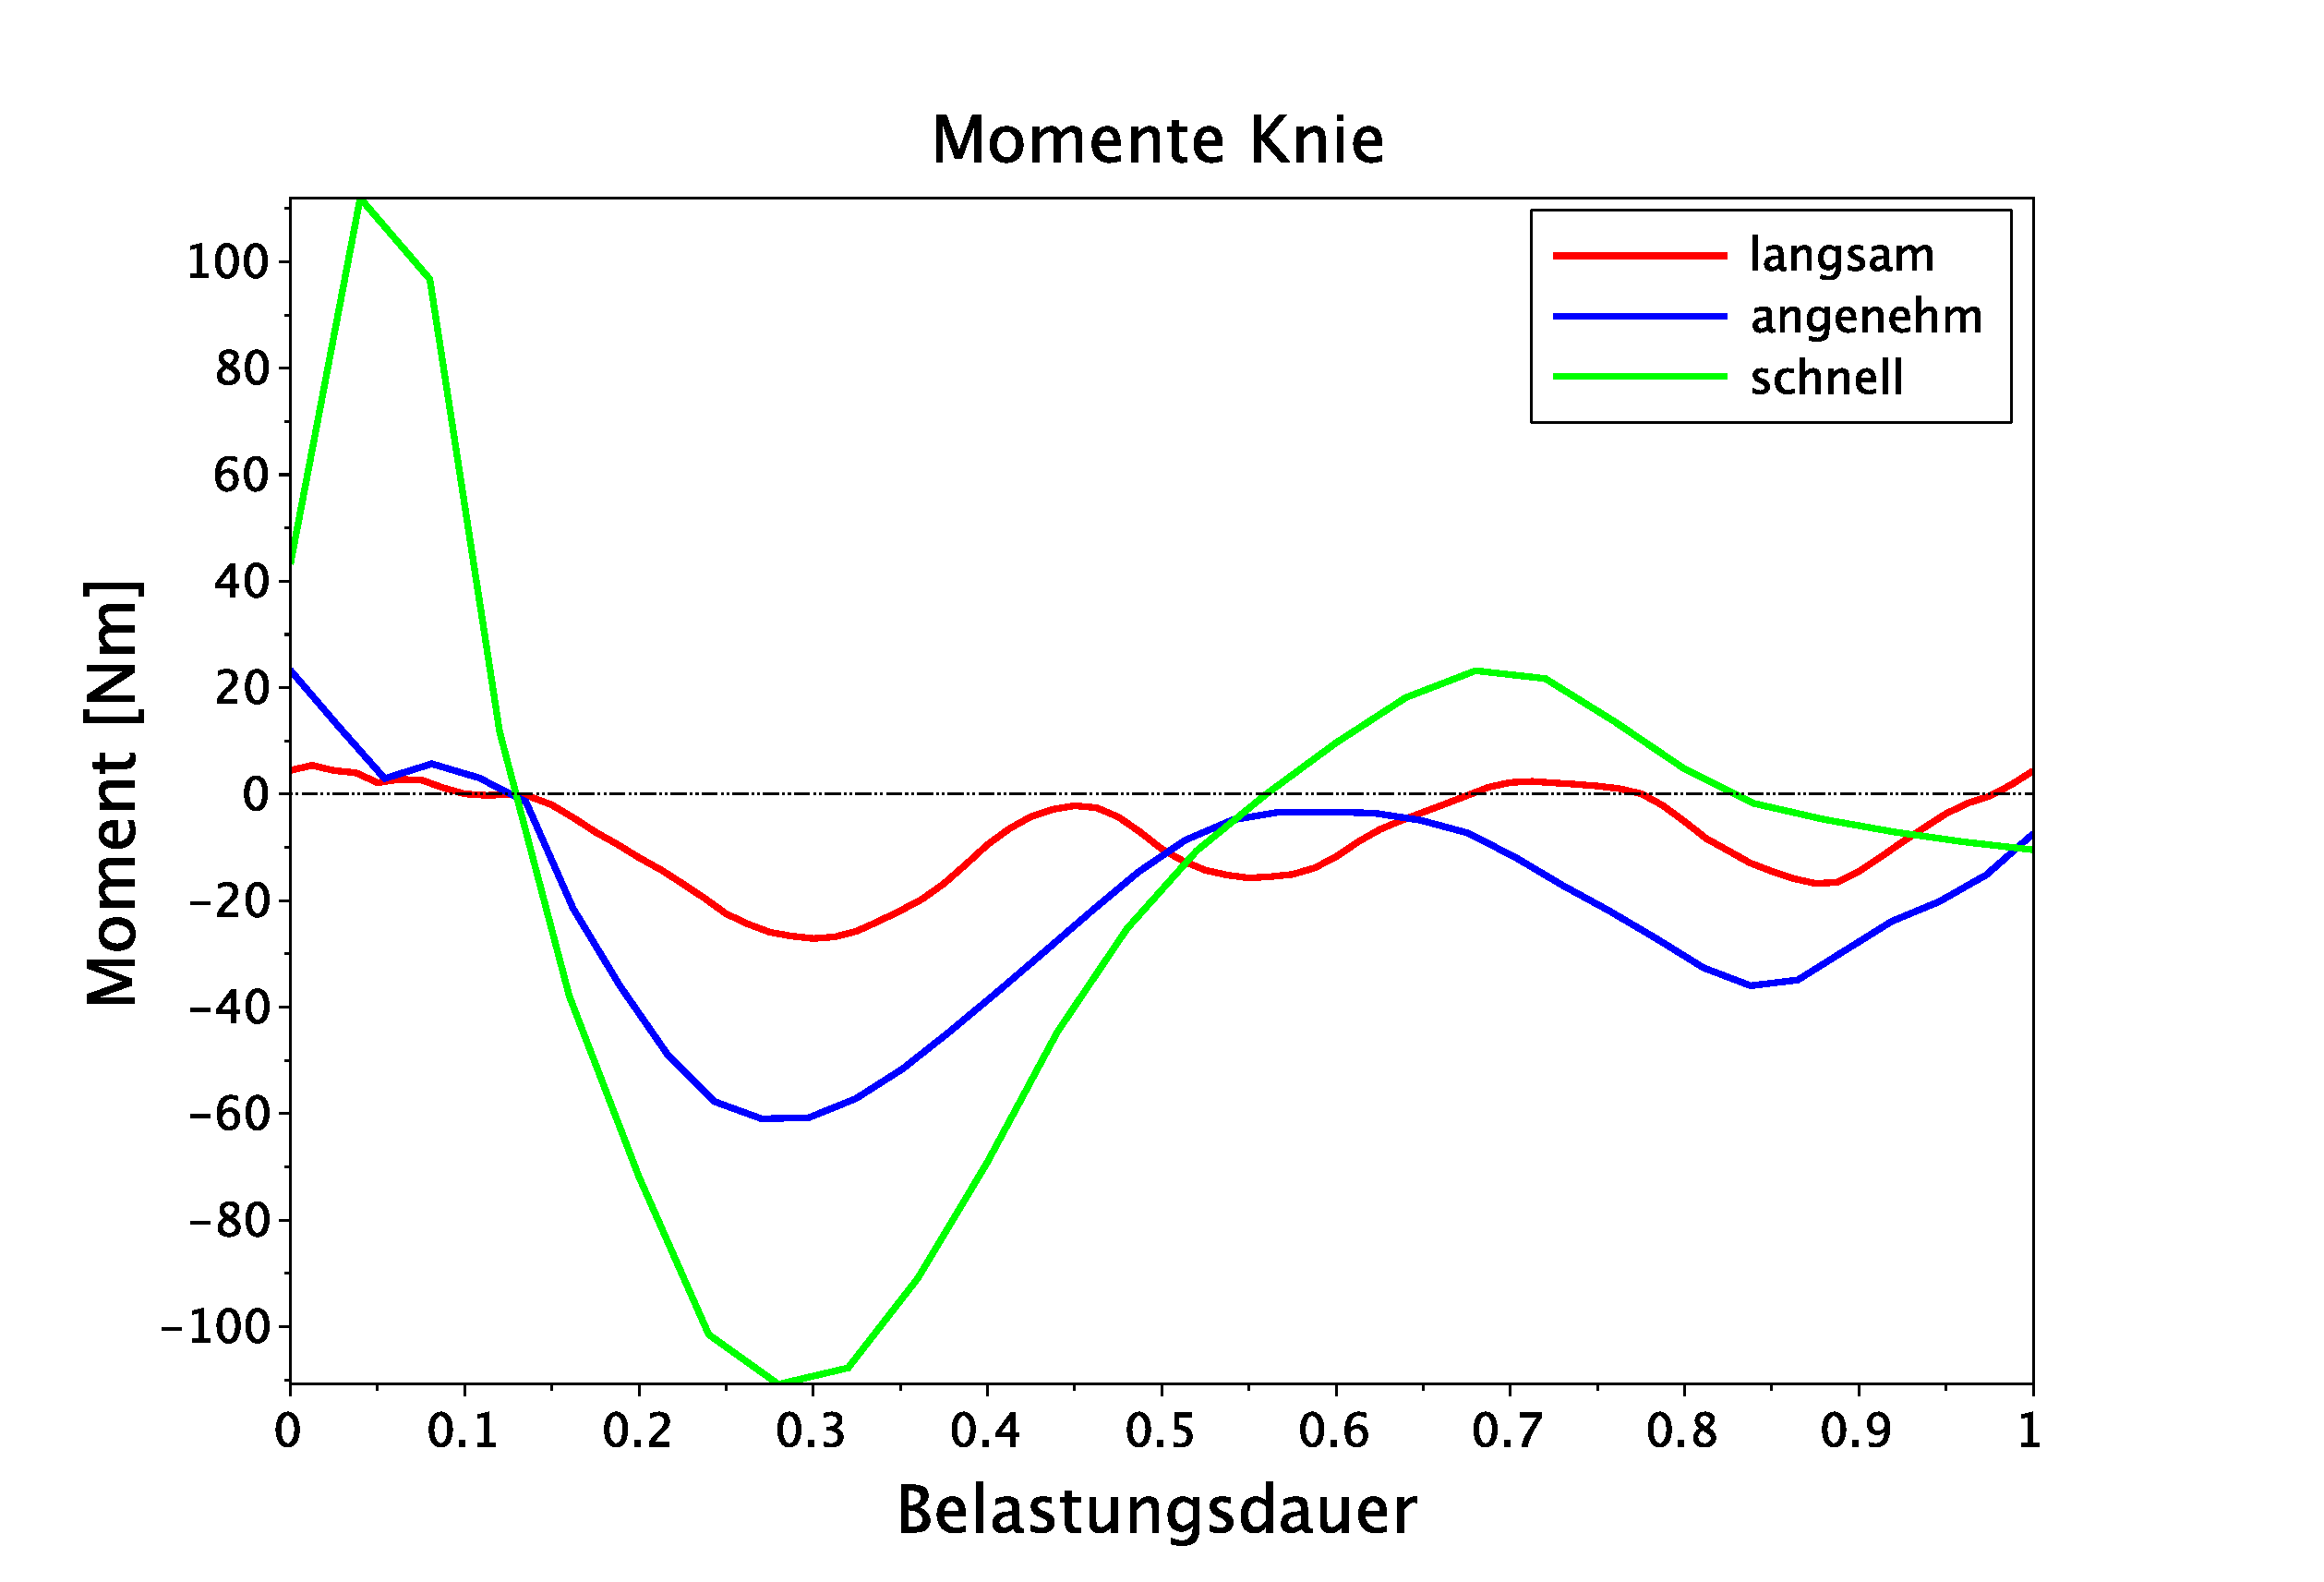
\includegraphics[width=0.7\linewidth]{bilder/ergebnisse/momente_knie.pdf}
	\caption[Bodenreaktionskräfte]{Verlauf von $F_x$, $F_y$ und $M$ während der Standphase.}
	\label{fig:knee_m}
\end{figure}


\subsection{Vergleich Laufband und Laufstrecke}
\textbf{Vergleich Laufstrecke und Laufband}\\
Mithilfe von Winkelmessungen des Oberkörpers, Arme und Beine können die beiden Gangarten verglichen und analysiert werden\\
Die Armbewegungen, welcher in \autoref{fig:vergleich_hand} zu sehen ist, lassen einen Vergleich zwischen den beiden Versuchsaufbauten, sowie unter den Geschwindigkeiten zu. In blautönen eingetragen sind dabei die Versuche auf dem Laufband, in rottönen die auf der Laufstrecke. \\
Die x- und y-Achse geben den horizontalen, bzw. vertikalen Abstand zum Nacken wieder. Je weiter links unten eine Trajektorie sich befindet, umso ausgestreckter ist der Arm.\\
Auf dem Laufband ist die Amplitude des Handgelenkes bei der niedrigsten eingezeichneten Geschwindigkeit von 2\,\kmh (cyan) 0,52\,m, die bei 4\,\kmh beträgt 0,57\,m und die der höchsten Geschwindigkeit (7\,\kmh, dunkelblau) 0,62\,m. 

0,35, 0,10, 0,73


\begin{figure}[h!]
	\centering
	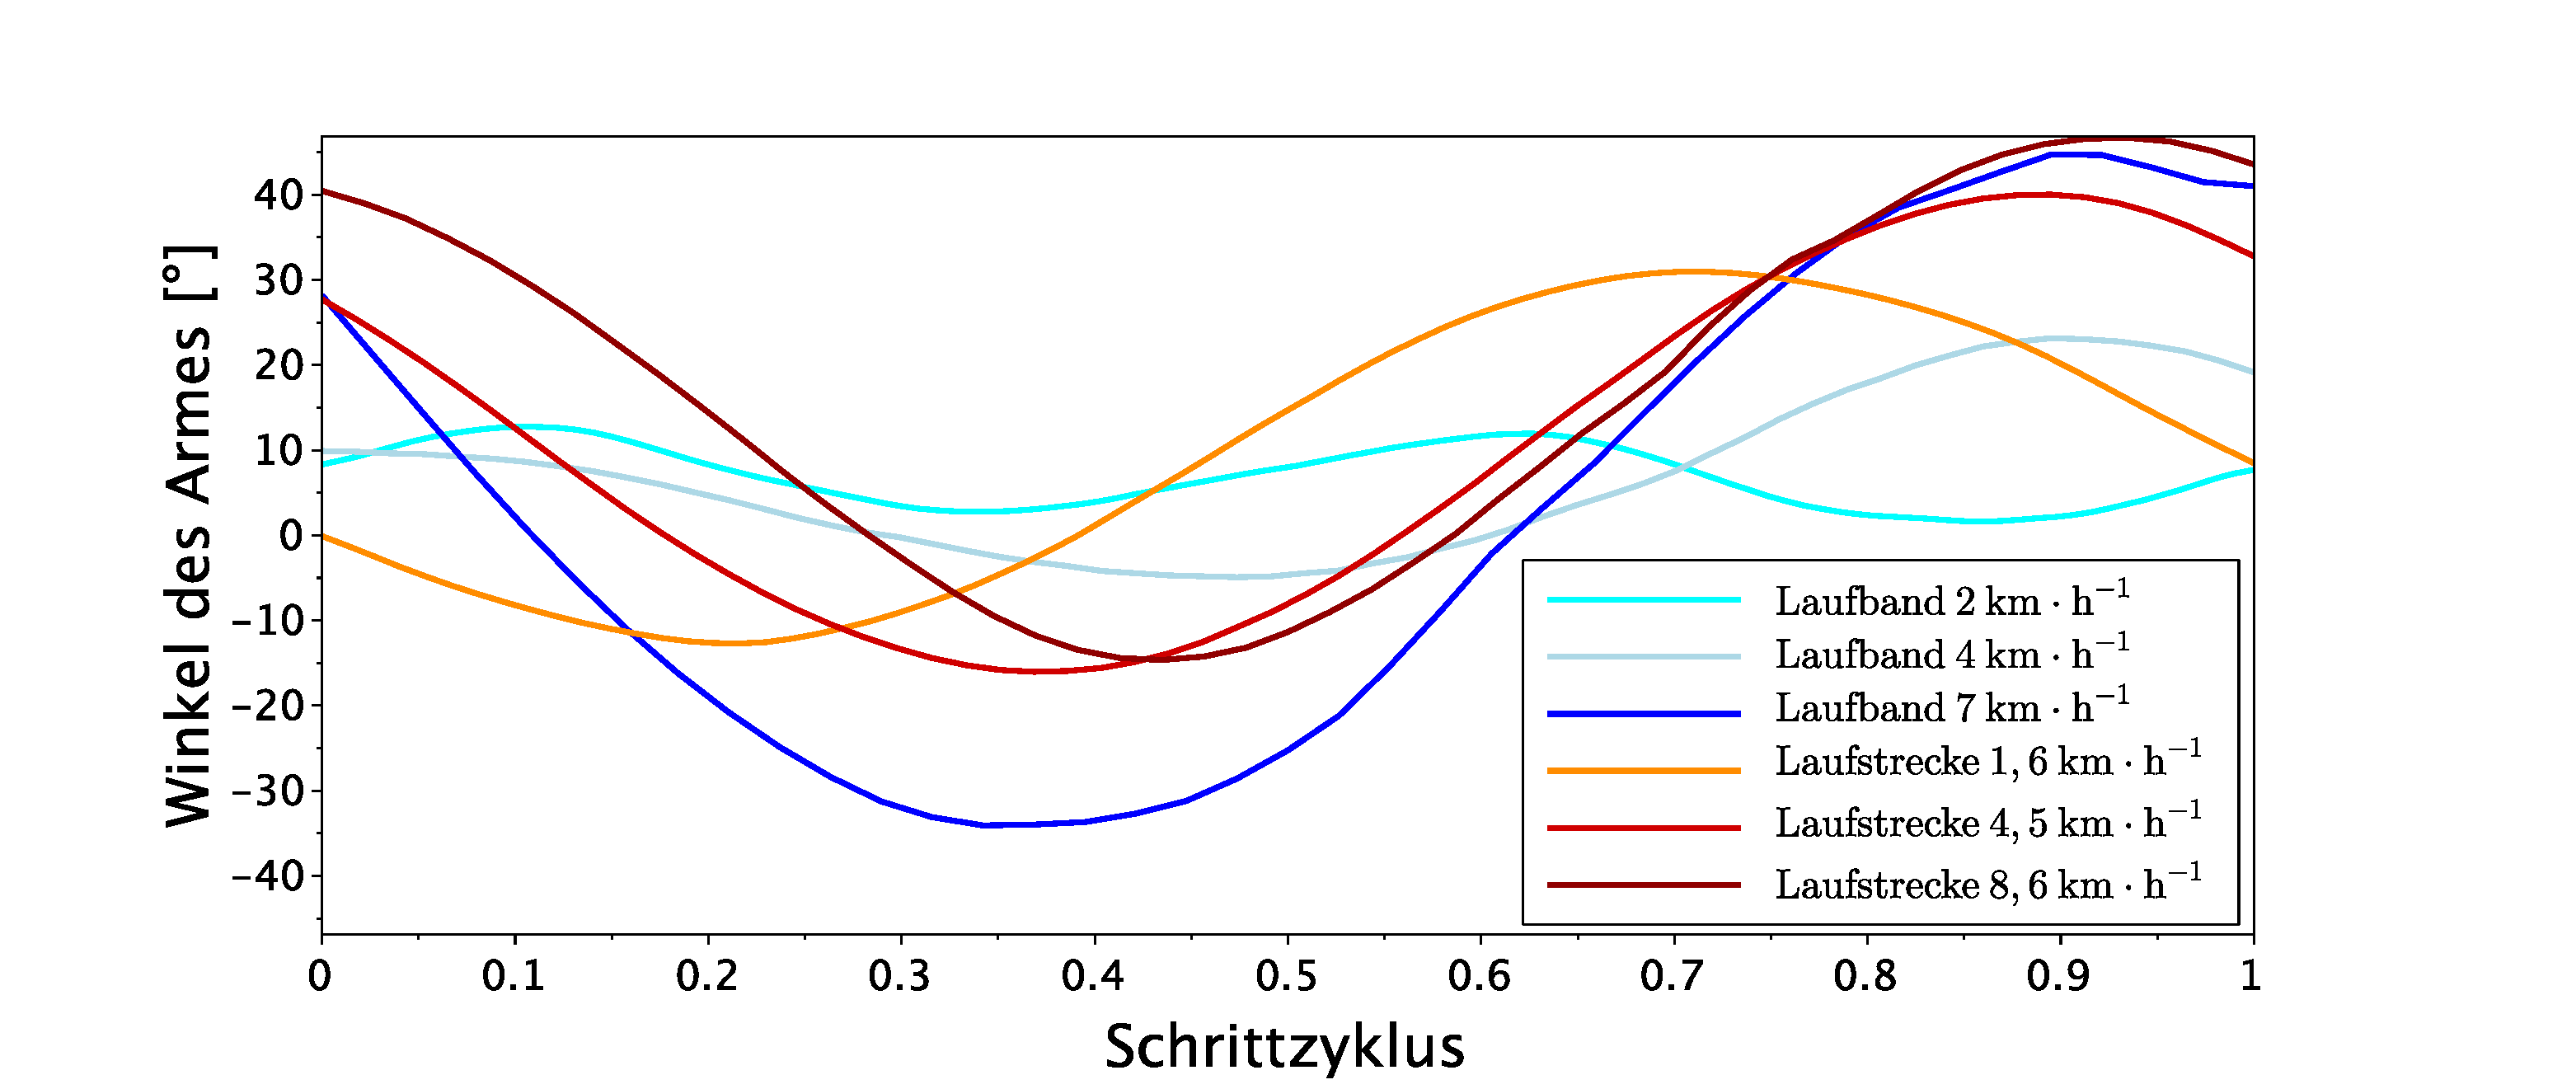
\includegraphics[width=1\linewidth]{bilder/ergebnisse/armschwung_winkel.pdf}
	\caption[Handtrajektorie]{Bewegung des Handgelenks, relativ zum Nacken. Negative x-Werte entsprechen einem Vorschwung, positive Werte einem Zurückschwingen. Auf der Laufstrecke ändert sich die relative Haltung des Handgelenks nach einem Schrittzyklus.}
	\label{fig:vergleich_hand}
\end{figure}

Ein weiterer Vergleich zwischen den Experimenten ist in \autoref{fig:vergleich_oberkörper} zu sehen. Eingetragen sind die relativen Neigungswinkel der Strecke Hüfte - Nacken. Ein Winkel von null Grad entspricht dem aufrechten Stehen, wenn der Nackenmarker senkrecht über dem Hüftmarker steht. Bei positiven Winkeln ist der Nackenmarker in Laufrichtung weiter vorne, bei negativen weiter hinten. Die Werte des Laufbandversuchs sind in Blautönen eingefärbt (cyan, graublau, dunkelblau), die Laufstreckenergebnisse in Rottönen (orange, rot, rotbraun). Allen Kurven gemein ist, dass während des Schrittzykluses der Winkel abfällt und daraufhin wieder ansteigt. Das Minimimum von vier Kurven liegt jeweils bei etwa 50\,\% der Schrittdauer. Einen klaren Unterschied zeigen die jeweils langsamsten Gehgeschwindigkeiten (cyan und orange), mit einer geringen Amplitude von 4,74 und 4,41 Grad und einem periodischen Wanken. Die größten Amplituden finden sich bei den höchsten Geschwindigkeiten mit 12,74 und 10,24 Grad für 7 (dunkelblau), beziehungsweise 8,6\,\kmh.

\begin{figure}[h!]
	\centering
%	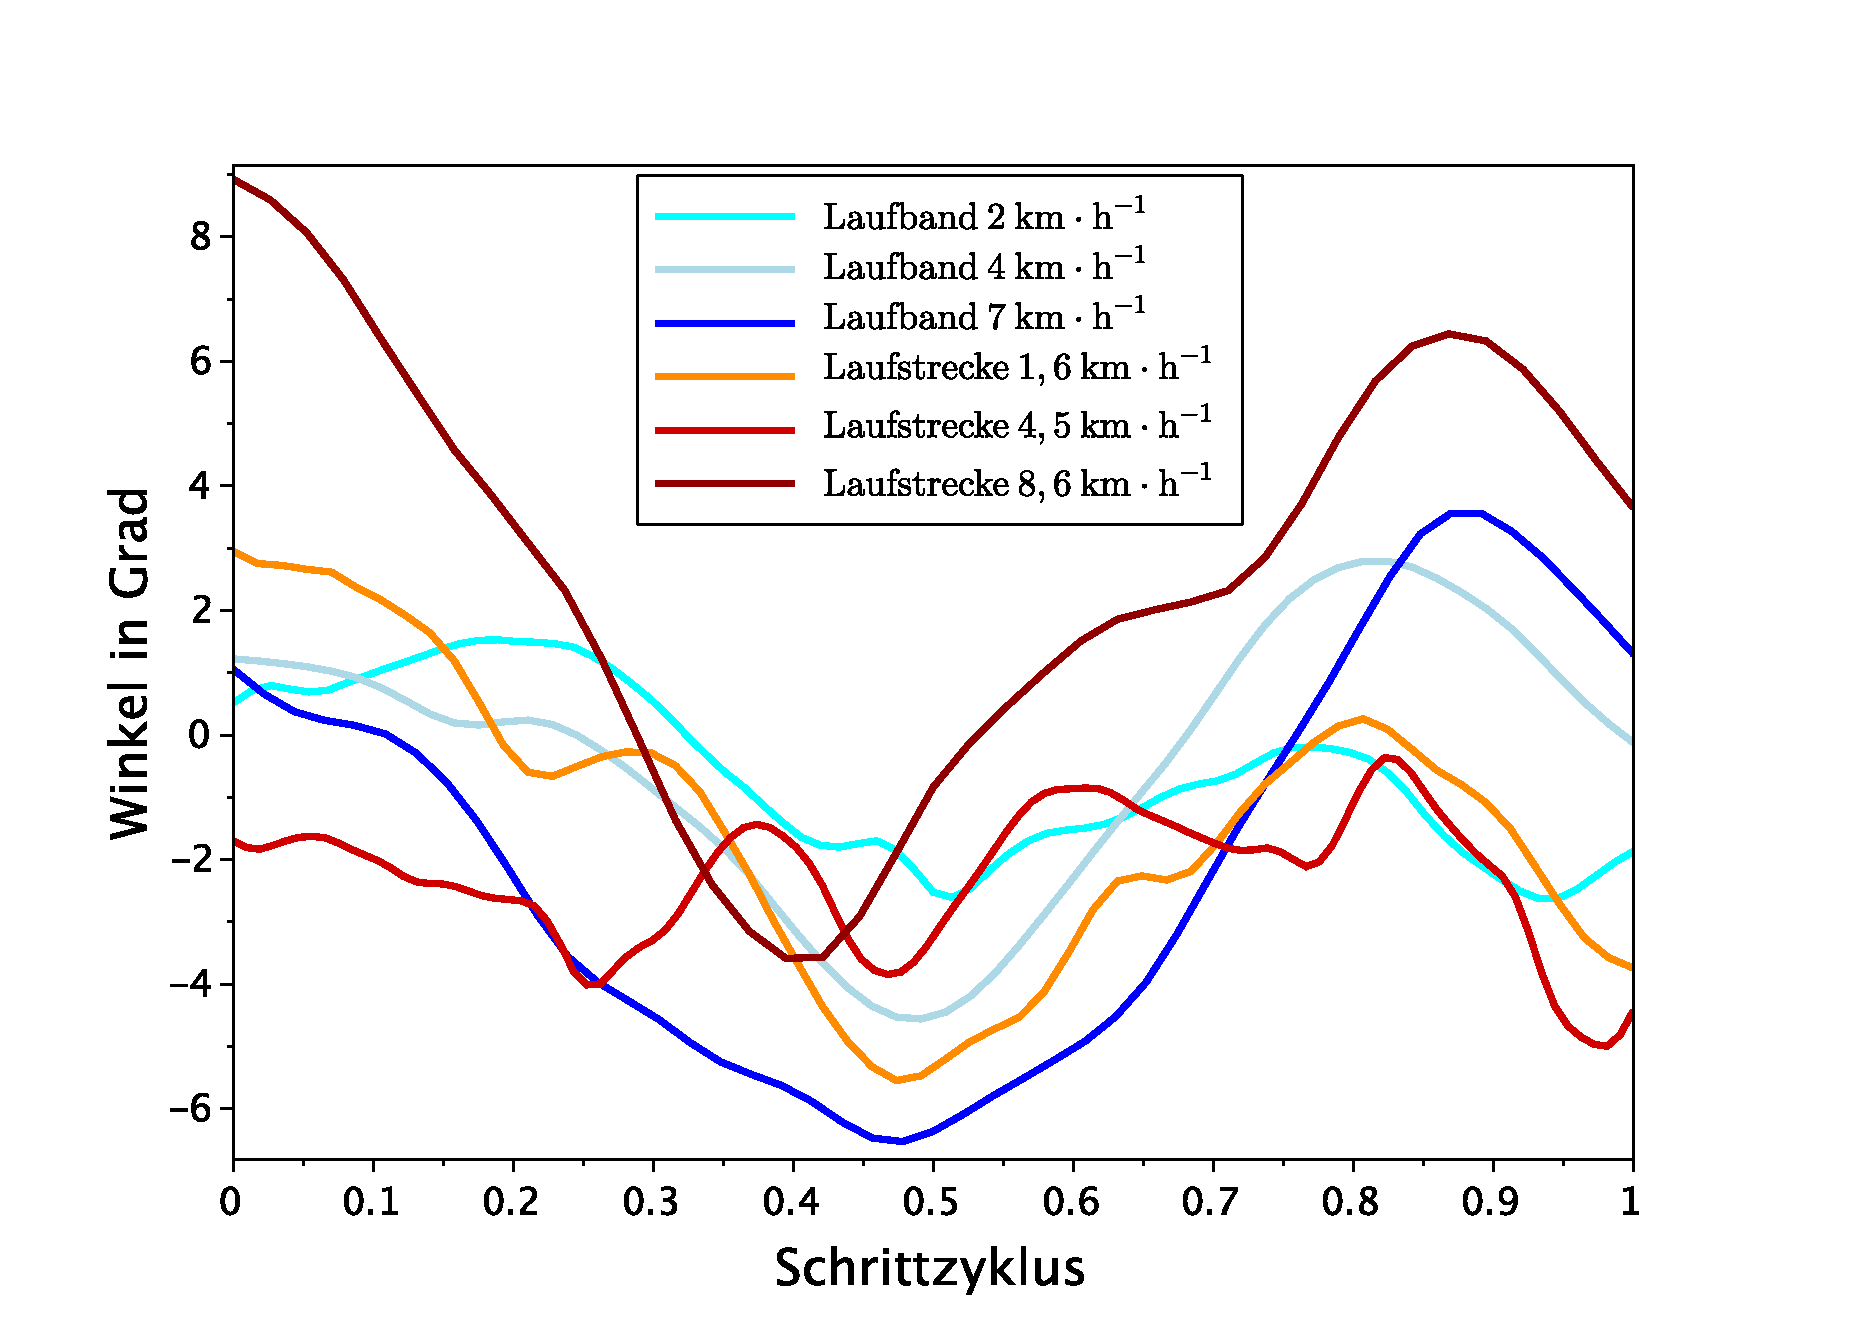
\includegraphics[width=0.7\linewidth]{bilder/ergebnisse/winkel_vergleich.pdf}
	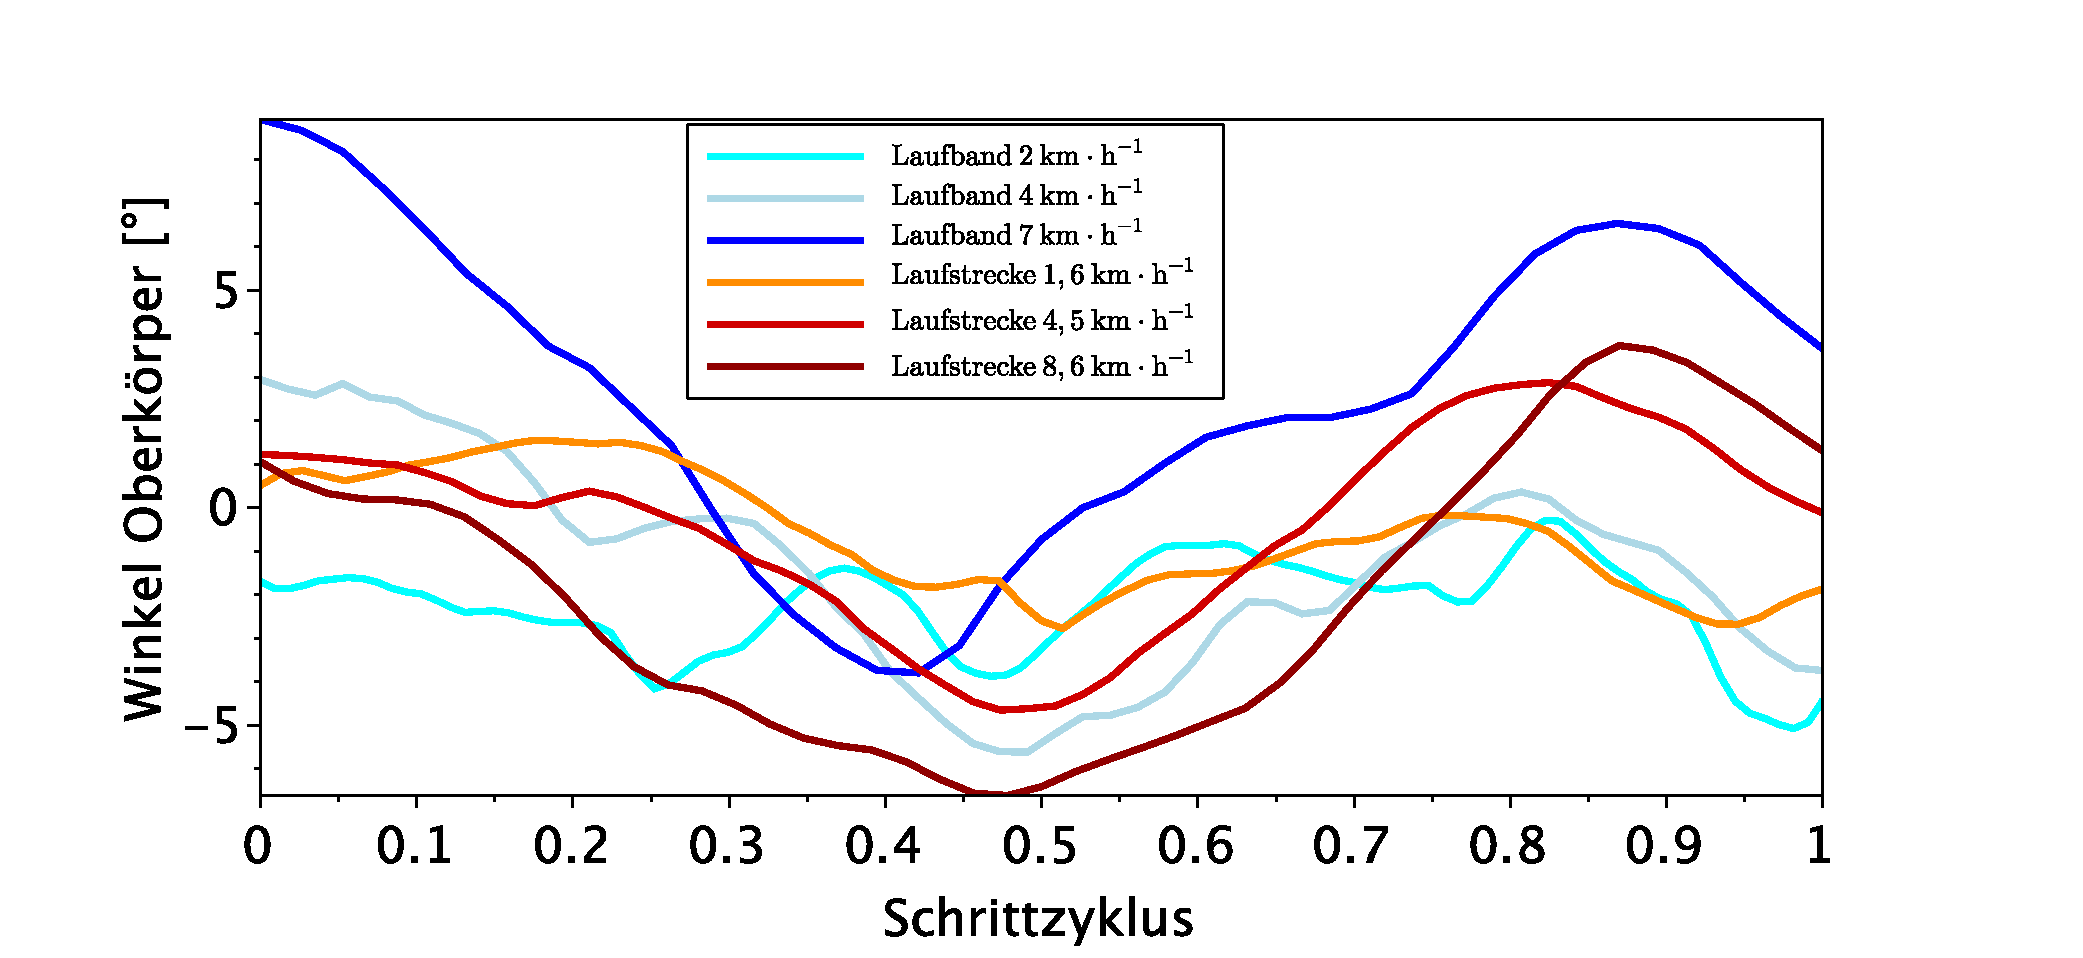
\includegraphics[width=1\linewidth]{bilder/ergebnisse/back_angle.pdf}
	\caption[Bodenreaktionskräfte]{Neigung des Oberkörpers. Negative Werte entsprechen einem Zurücklehnen, positive Werte einem Vorlehnen. Winkelwerte wurden mit einem gleitenden Mittelwert in zwei Durchläufen geglättet.}
	\label{fig:vergleich_oberkörper}
\end{figure}

\section{Diskussion}
\subsection{Durchgeführte Experimente}
Um die Biomechanik des Gehens zu untersuchen, wurden zwei Versuche durchgeführt: Das stationäre Gehen auf einem Laufband und das Gehen über eine Laufstrecke. Ersteres bietet die Möglichkeit, die Kinematik des Gehens eingehend zu studieren. Stationär deshalb, da die Fortbewegung innerhalb des Raumes gleich null ist. Der Proband kann so seinen Laufrhythmus finden, die Geschwindigkeit kann von außen vorgegeben werden und es können mehrere Schritte hintereinander aufgezeichnet werden. Das Gehen auf der Laufstrecke ermöglicht es, während eines Bodenkontaktes auf der eingebauten Waage die Bodenreaktionskräfte in drei Raumrichtungen aufzunehmen. Gekoppelt mit einer gleichzeitig Laufenden Kamera lassen sich Video- und Kraftmessungen zusammenführen und mit der Methode der inversen Dynamik können die wirkenden Kräfte in den Gelenken des Beines rekonstruiert werden. \\
Bei dem Probanden handelt es sich um einen 24 jährigen Mann, ohne bekannte Gelenkschäden, Haltungsschäden oder anderweite Beeinträchtigungen. 
\textbf{AUSWIRKUNGEN VON SCHUHWERK AUF GEHSTIL?}


\subsection{Bodenreaktionskräfte}
In \autoref{fig:brk} sind die beim angenehmen Gehen auftretenden Bodenreaktionskräfte eingezeichnet und zusätzlich die Belastungsphasen, wie beschrieben in perry2003gang eingetragen. Zum Ende der terminalen Schwungphase befindet sich die Ferse etwa 1\,cm über dem Boden und fällt dann im freien Fall auf den Boden: Es kommt zum initialen Kontakt, erkennbar am Anstieg bist zum durch den Pfeil gekennzeichneten Hubbel in \autoref{fig:brk} . Der Fuß rollt dabei über die Ferse ab und bereits bevor die Belastungsantwort abgeschlossen ist (erstes Maximum) hat der gesamte Fuß Kontakt. Durch die Bewegung des Körperschwerpunktes in Richtung Boden sollte die auftretende vertikale Kraft etwa 110\,\% des Körpergewichtes ausmachen, was hier jedoch nicht ganz erreicht wird. Gleichzeitig 
\begin{figure}[h!]
	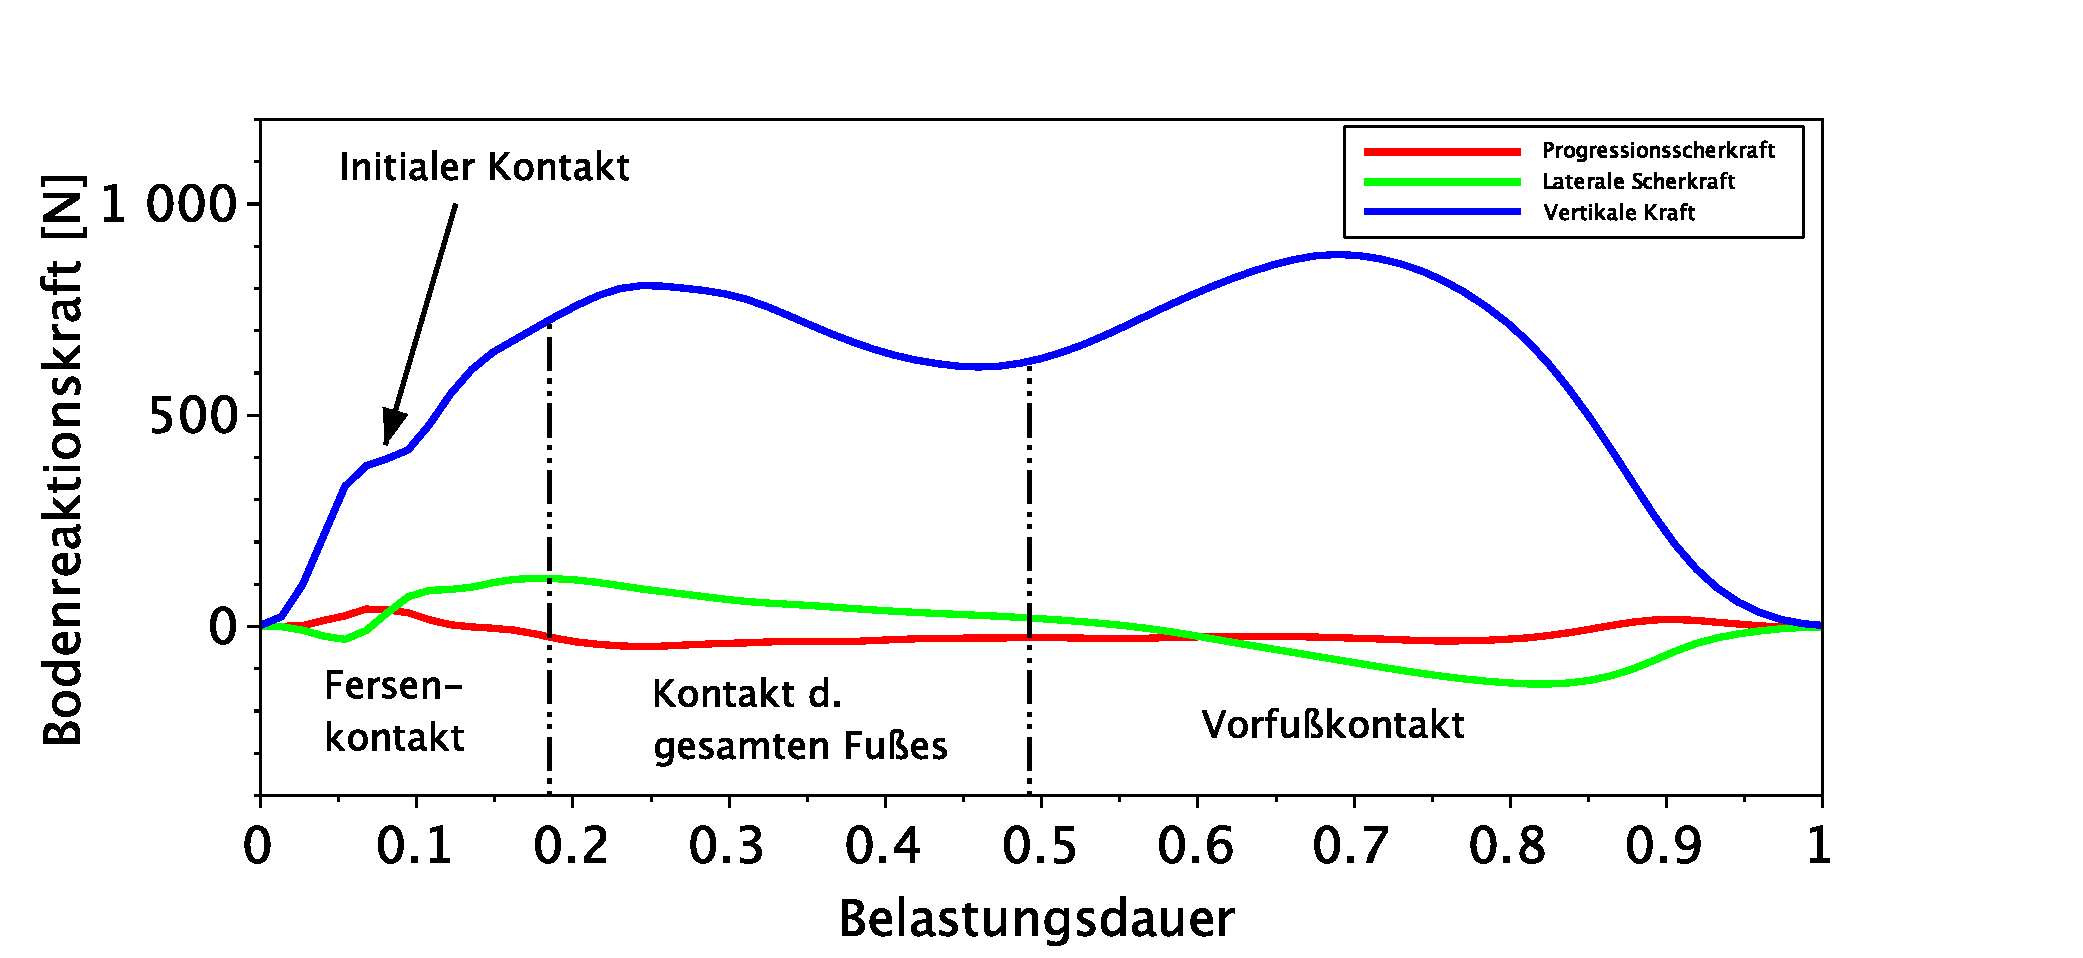
\includegraphics[width=\linewidth]{bilder/Ergebnisse/brk_annotations.pdf}
	\caption{Bodenreaktionskräfte}
	\label{fig:brk}
\end{figure}



\subsection{Vergleich Laufband}
Im Unterschied zum Laufband kommt es zu einer realen Fortbewegung im Raum, was die Frage aufwirft, ob diese beiden Bewegungsformen überhaupt vergleichbar sind. Macht es einen Unterschied, ob sich eine Person relativ zu einem bewegten Untergrund mit einer gewissen Geschwindigkeit bewegt, von einem fixen äußeren Bezugssystem (stationäre Kamera) jedoch keine Geschwindigkeit aufzuweisen scheint, oder ob sich die Person mit derselben Geschwindigkeit auf einem fixen Untergrund bewegt, betrachtet von einem bewegten Bezugssystem (bewegte Kamera).\\
Es sei vorweg genommen, dass die Beantwortung dieser Frage eine statisch relevante Methodik erfordert und die Versuchsaufbauten soweit optimiert werden müssen, dass einzig das Bezugssystem sich ändert. Dies würde bedeuten, dass die Laufstrecke so lang ist, dass keine Beschleunigungs oder Bremsvorgänge während der Aufnahme stattfinden und eine konstante, vorgegebene Geschwindigkeit eingehalten wird, wie dies auf dem Laufband der Fall ist.\\
Im Rahmen der vorliegenden Arbeit war eine solche Methodik jedoch nicht durchführbar, weshalb die folgenden Überlegungen theoretischer Natur sind, gestützt von einem Datensatz ohne Anspruch auf statistische Relevanz. 







\paragraph*{Fazit}
\paragraph*{Ausblick}


%\begin{spacing}{0.05}
%\thispagestyle{plain}
%\section{Quellenverzeichnis}
%\pagestyle{scrheadings}
%\ohead{Quellenverzeichnis}
%\bibliographystyle{chicago}
%\bibliography{bibliographie}
%\end{spacing}

\section{Literatur}
Das Literaturverzeichnis ist nach folgendem Schema zu gestalten: (siehe Skritp)\\


%%---------------------------------------------------------
%% Anhang, falls erforderlich
%%---------------------------------------------------------
\appendix                %% appendix ist keine Umgebung!

\pagenumbering{roman}
\setcounter{page}{1}
\section*{Anhang}%


Im Folgenden sind die verwendeten Gleichungen aufgeführ, die Tiefgestellten Buchstaben A, K, H und W indexieren Knöchel, Knie, Hüfte und die Waage -  F, B, und O stehen für die Segmente Fuß, Unterschenkel und Oberschenkel\\
\begin{align*}
& \quad \text{\textbf{Knöchel}}\\
& F_{x, A} =  m_F \cdot \ddot{x}_F - F_{x, W} \\
& F_{y, A} =  m_F \cdot (\ddot{y}_F - g) - F_{y, W} \\
& M_{A} =  J_{0, F} \cdot \ddot{\alpha}_F  \\
& \qquad - F_{y, A} (x_A, - x_F) - F_{x, A} (y_A, - y_F)\\
& \qquad - F_{y, W}(x_W - x_F) -  F_{x, W}(y_F - y_W)	\\
%		
&\quad \text{\textbf{Knie}}\\
& F_{x, K} =  m_B \cdot \ddot{x}_B - (-F_{x, A}) \\
& F_{y, K} =  m_B \cdot (\ddot{y}_B - g) - (-F_{y, A}) \\
& M_{K} =  J_{0, B} \cdot \ddot{\alpha}_B  \\
& \qquad - (-F_{y, K}) (x_K, - x_B) - (-F_{x, K}) (y_K, - y_B)\\
& \qquad- (-F_{y, A})(x_A - x_B) -  (-F_{x, A})(y_B - y_A)	\\
%		
& \quad \text{\textbf{Hüfte}}\\
& F_{x, H} =  m_O \cdot \ddot{x}_O - (-F_{x, K}) \\
& F_{y, H} =  m_O \cdot (\ddot{y}_O - g) - (-F_{y, K}) \\
& M_{H} =  J_{0, O} \cdot \ddot{\alpha}_O  \\
& \qquad - (-F_{y, H}) (x_H, - x_O) - (-F_{x, H}) (y_H, - y_O)\\
& \qquad- (-F_{y, K})(x_K - x_O) -  (-F_{x, K})(y_O - y_K)				
\end{align*}
\end{document}